\documentclass[conference]{IEEEtran}
\IEEEoverridecommandlockouts
\usepackage{cite}
\usepackage{amsmath,amssymb,amsfonts}
\usepackage{algorithmic}
\usepackage{graphicx}
\usepackage{textcomp}
\usepackage{xcolor}
\usepackage{booktabs}
\usepackage{array}
\usepackage{url}
\usepackage{tikz}
\usetikzlibrary{shapes.geometric,arrows.meta,positioning}
% ---------- TikZ styles ----------
\tikzset{
  term/.style   = {circle, draw, fill=blue!30!gray!80, text=white,
                   font=\normalsize\bfseries, minimum size=0.95cm, align=center},
  proc/.style   = {draw, fill=blue!8, rounded corners=2pt,
                   font=\normalsize, minimum width=3.6cm,
                   minimum height=0.8cm, align=center},
  procN/.style  = {draw, fill=blue!8, rounded corners=2pt,
                   font=\normalsize, minimum width=2.6cm,
                   minimum height=0.95cm, align=center},
  procW/.style  = {draw, fill=blue!8, rounded corners=2pt,
                   font=\normalsize, minimum width=4.0cm,
                   minimum height=0.8cm, align=center},
  dec/.style    = {diamond, draw, fill=blue!5,
                   font=\normalsize, minimum width=2.8cm,
                   minimum height=1.0cm, aspect=1.8, align=center},
  arr/.style    = {-Stealth, thick},
  arrthin/.style= {-Stealth, semithick}
}
% ---------------------------------
\def\BibTeX{{\rm B\kern-.05em{\sc i\kern-.025em b}\kern-.08em
    T\kern-.1667em\lower.7ex\hbox{E}\kern-.125emX}}
\begin{document}
\title{StudyMate: An Adaptive RAG Teaching Assistant\\
with YouTube Persona-Driven Explanation for Students}
\author{
\IEEEauthorblockN{Dr.\ B Swathi}
\IEEEauthorblockA{Dept.\ of CSE (Data Science)\\
New Horizon College of Engineering\\
Bengaluru, India\\
basawarajus@newhorizonindia.edu}
\and
\IEEEauthorblockN{Monish V}
\IEEEauthorblockA{Dept.\ of CSE (Data Science)\\
New Horizon College of Engineering\\
Bengaluru, India\\
1nh23cd092@newhorizonindia.edu}
\and
\IEEEauthorblockN{Manprit}
\IEEEauthorblockA{Dept.\ of CSE (Data Science)\\
New Horizon College of Engineering\\
Bengaluru, India\\
1nh23cd087@newhorizonindia.edu}
\and
\IEEEauthorblockN{Sinchana R M}
\IEEEauthorblockA{Dept.\ of CSE (Data Science)\\
New Horizon College of Engineering\\
Bengaluru, India\\
1nh23cd165@newhorizonindia.edu}
\and
\IEEEauthorblockN{Sushmitha Yadwad}
\IEEEauthorblockA{Dept.\ of CSE (Data Science)\\
New Horizon College of Engineering\\
Bengaluru, India\\
1nh23cd172@newhorizonindia.edu}
}
\maketitle
\begin{abstract}
Personalised academic help is scarce where it is needed most. In many
engineering colleges a single teacher is responsible for roughly a
hundred students, learners who think in a language other than English
are left with tools that only speak English, and none of the general
assistants a student can reach actually know the syllabus being taught.
This paper argues that closing these gaps requires more than a better
answer engine---it requires answers that a student is willing to read,
delivered in a voice the student already trusts. We present
\textit{StudyMate}, a Telegram-based teaching assistant built on
Retrieval-Augmented Generation (RAG) that grounds every reply in
institution-specific material and, uniquely, can reproduce the
explanatory style of a YouTube educator the student already follows.
The significance of the work is twofold. First, StudyMate unifies nine
capabilities---curriculum-grounded tutoring, five-year Previous Year
Question (PYQ) trend mining, Bloom's-graded mock papers, an
exam-aware study planner, persistent dialogue memory, bilingual voice,
encrypted storage, an adaptive pedagogy layer, and instructor-style
personalisation---that prior systems only ever delivered one or two at
a time. Second, its \emph{YouTube Transcript Persona Engine}
(Module~12) introduces persona-conditioned generation to educational
RAG, a capability we did not find in any reviewed system. Because the
platform is being submitted as a design-and-architecture contribution,
we report the evaluation protocol and the acceptance thresholds that
will decide success rather than post-hoc numbers: RAGAS Faithfulness
$\geq 0.85$, Answer Relevance $\geq 0.80$, faculty-validated domain
accuracy $\geq 85\%$, a Persona Style Consistency score $\geq 0.78$,
and a Technology Acceptance Model (TAM) Perceived Usefulness
$\geq 4.0/5.0$ over a cohort of $N \geq 30$ students. The paper also
details how hallucinations are contained, how the design reduces
computational and energy cost, and where the study's validity is most
at risk.
\end{abstract}
\begin{IEEEkeywords}
Retrieval-Augmented Generation, Educational Chatbot, Telegram Bot,
LangChain, Qdrant, MiniLM, Bloom's Taxonomy, RAGAS, TAM, Ollama,
Multilingual NLP, Study Planner, YouTube Transcript, Persona Engine,
Sustainable AI
\end{IEEEkeywords}
%------------------------------------------------
\section{Introduction}
%------------------------------------------------
Anyone who has watched a batch of students prepare for end-semester
examinations recognises the same scramble every year. Students leaf
through old question papers by hand, trying to guess which topics will
reappear. They queue outside a staff room where one lecturer is
already stretched across a hundred learners. When neither works, they
fall back on a general chatbot that has never seen their syllabus and
answers with breezy confidence about the wrong course. Not one of
these routes scales, and none of them reaches the students who learn
best when a concept is explained the way a familiar teacher would put
it rather than in the flat register of a language model~\cite{lauber2025}.

The pedagogical stakes are not small. Bloom's classic 1984 study found
that one-to-one tutoring lifts outcomes by about two standard
deviations over ordinary classroom teaching~\cite{bloom1984}. Large
language models (LLMs) are the first technology that could plausibly
approximate that attention for a whole cohort at once. The catch is
well known: a model that leans only on its pre-trained weights will
state things that sound right but drift away from the actual course
material~\cite{lewis2020}. RAG was introduced precisely to fix
this---it forces the model to answer from passages retrieved at query
time~\cite{lewis2020}. Yet even a faithfully grounded RAG reply is
still written in the model's own voice, not in the voice of the
YouTube educator a particular student finds easiest to follow. That
last gap is the one this paper sets out to close.

StudyMate's answer is its twelfth module, the YouTube Transcript
Persona Engine. A teacher or a student registers the URLs of lecture
videos tied to the course; the system pulls the transcripts, timestamps
them, and indexes them into a dedicated Qdrant collection. When a
question arrives, passages from the matching educator are injected into
the prompt together with a short style descriptor distilled from that
educator's own words. What comes back is a reply that is grounded in
the institution's material yet phrased in the recognisable manner of
the instructor the student already trusts. To our knowledge no earlier
educational RAG system has combined corpus-grounded retrieval with
transcript-level persona conditioning, and this combination is the
paper's central claim to novelty.

The persona engine does not stand alone. It sits on top of a design
that tackles eight further problems which tend to appear together in
resource-constrained classrooms and which, taken as a set, no single
prior system resolves: the roughly 100:1 student-to-faculty ratio,
English-only tooling, PYQ archives that nobody mines, the lack of any
exam-aware scheduling, chatbots that forget everything between
sessions, conversation logs kept in the clear, the absence of
Bloom's-aligned practice papers, and a one-size-fits-all explanation
style. Fig.~\ref{fig:flowchart} traces a single message from a
student's phone through the whole pipeline.

The specific contributions of this work are the following.
\begin{itemize}
    \item A twelve-module RAG architecture grounded in
          institution-specific syllabi, module notes, PYQ corpora, and
          YouTube lecture transcripts.
    \item A YouTube Transcript Persona Engine (Module~12) that
          conditions generation on a registered educator's style
          fingerprint, so that answers feel familiar to students
          already used to that instructor's teaching voice.
    \item A TF-IDF PYQ trend engine that measures topic recurrence and
          mark-category distribution across five academic years.
    \item A Bloom's-taxonomy mock-paper generator that reproduces the
          official university question-paper format.
    \item An exam-date-aware, weak-topic-weighted study planner.
    \item An adaptive learner-modelling layer that tunes response
          depth, explanation style, and Socratic guidance to each
          student's demonstrated ability.
    \item Bilingual voice I/O carried over MTProto transport encryption.
    \item An evaluation protocol combining RAGAS, a new Persona Style
          Consistency metric, and TAM over $N \geq 30$ students, with
          an explicit treatment of hallucination control, sustainability,
          and threats to validity.
\end{itemize}

\noindent\textit{Note on integrity.} A plagiarism and AI-content
similarity report generated with the conference-recommended tool is
submitted as supplementary material alongside this manuscript; the
prose here has been authored and revised by the student team.

%------------------------------------------------
\section{Literature Survey}
%------------------------------------------------
We group the prior work into eight strands and, for each, state plainly
how StudyMate builds on or departs from it. The comparison is not meant
to diminish these systems---most are strong within their scope---but to
locate the specific opening this paper fills.

\subsection{Didactic Alignment of RAG Chatbots}
Lauber, Martin, and Pampel~\cite{lauber2025} were among the first to
tie RAG chatbot design to formal pedagogy, pairing Reinmann's Didactic
Design model with Cognitive Apprenticeship theory and defining three
assistant roles: Learning Instructor, Learning Partner, and Learning
Assistant. They validated the idea on Flowise and LangChain inside a
single German computer-science course. Their role taxonomy directly
informs StudyMate's prompt design (Section~V-C); where we diverge is
scope and voice---their framework was never tested outside German, ran
no TAM study, ignored multilingual learners, and had no way to shape
an answer around an external educator's manner of speaking.

\subsection{RAG Architecture Survey for Education}
Teixeira, Sonkaya, and Georgieva~\cite{teixeira2025} benchmarked vector
stores and embedding models on educational workloads: Qdrant won on
throughput and latency, MiniLM and MPNet gave the best speed-accuracy
trade-off, and RAGAS emerged as the sensible production evaluator.
These findings are load-bearing for us---they justify our choice of
Qdrant and \texttt{all-MiniLM-L6-v2}. The gap is that their study is a
paper benchmark with no running prototype, no learners, and no notion
of institution-specific or persona-conditioned generation.

\subsection{LLM-Driven Chatbot in Higher Education}
Neumann et al.~\cite{neumann2025} fielded MoodleBot by joining GPT-4 to
Weaviate for a German database course, reporting 88\% accuracy and
strong TAM scores (PU\,=\,4.46, PEOU\,=\,4.60) across 47 participants.
Their TAM instrument is a useful template for ours. But MoodleBot is
one course in one language, leans on cloud inference with the attendant
privacy cost, and offers nothing for PYQ-based preparation, adaptive
explanation, or persona conditioning---exactly the axes StudyMate adds.

\subsection{Knowledge Graph-Enhanced RAG}
KG-RAG~\cite{dong2025} strengthens retrieval with a DeepSeek-V3
knowledge graph for finance education and improves multi-hop reasoning.
Its weakness is maintenance: syllabi change every year, and keeping a
curated triple store in step with them is hard to sustain. We therefore
keep the knowledge layer as re-indexable text and list KG augmentation
only as future work; KG-RAG also has no voice, no Telegram delivery,
and no persona layer.

\subsection{URAG: Hybrid RAG for University Admissions}
URAG~\cite{nguyen2025} cuts latency in admissions chatbots by routing
FAQ queries to keyword matching and hard queries to full RAG. The
routing idea inspired our lightweight command dispatcher, but URAG
answers admissions questions only---no concept tutoring, no per-student
memory, and no explanation personalisation.

\subsection{RAG-X: Intelligent Teaching Platform}
He et al.~\cite{he2025} built RAG-X from Dense Passage Retrieval, a
neural re-ranker, and a think--act--observe agent loop, reporting a
30.3\% UX gain over 62 students---a figure we use as a reference point
for expected impact. RAG-X, however, is Chinese-only, web-based, and
carries no voice, no multilingual reach, and no persona conditioning.

\subsection{ARIA: Multimodal RAG for Engineering Education}
ARIA~\cite{luo2026} pairs Docling, Nougat, and GPT-4 Vision to parse
multimodal engineering material at Johns Hopkins, hitting 97.5\%
accuracy with e5-large-v2 at 0.178\,s latency. It is excellent at
content retrieval and sets a high bar we acknowledge; it does not touch
PYQ-based exam prep, scheduling, voice, or instructor-style conditioning.

\subsection{Telegram Assessment, Greek-Language RAG, and RAGAS}
Gielis et al.~\cite{gielis2025} showed Telegram works as a
self-assessment platform, though with hand-written questions and no RAG,
multilingual input, or persona output. Koutsiaki et al.~\cite{koutsiaki2025}
compared six chunking strategies for a Greek university chatbot and
found sentence-preserving paragraph boundaries beat fixed windows---a
result we adopt verbatim in our ingestion pipeline. Es et al.~\cite{es2025}
introduced RAGAS as an LLM-as-judge evaluator for groundedness,
relevance, and context; we take RAGAS as our base and extend it with a
Persona Style Consistency metric. Broader surveys of educational
chatbots by Kuhail et al.~\cite{kuhail2023} and Wollny et al.~\cite{wollny2021}
reach a consistent verdict: most systems remain single-purpose, rarely
support regional languages, and almost never personalise their
explanatory style---the very shortfalls StudyMate targets.
Style-conditioned generation itself is well studied in open-domain
dialogue~\cite{li2023}, but has not been carried into grounded
educational RAG, which is where we position our contribution.

\subsection{Research Gaps}
Reading these strands together, five gaps recur across the literature
and motivate the present design.
\begin{enumerate}
    \item \textbf{Fragmented capability.} Systems solve one problem
          well---retrieval, or assessment, or scheduling---but no
          reviewed platform integrates tutoring, exam-trend mining,
          mock generation, planning, memory, and voice in one
          deployable service.
    \item \textbf{Language exclusion.} With the partial exception of
          Greek- and Vietnamese-specific studies, evaluation cohorts
          are English-fluent, leaving non-English learners
          under-served and under-measured~\cite{kuhail2023,wollny2021}.
    \item \textbf{Unmined institutional data.} PYQ archives, a rich
          predictor of what will be asked, are ignored by every system
          surveyed.
    \item \textbf{Privacy as an afterthought.} Cloud-inference designs
          send student data off-premises with no end-to-end guarantee.
    \item \textbf{Uniform, impersonal voice.} No educational RAG system
          adapts \emph{how} an answer is phrased to a trusted educator's
          style, despite evidence that familiarity lowers cognitive
          friction~\cite{zhao2024,li2023}.
\end{enumerate}
StudyMate is designed as a direct response to all five, with the fifth
gap---persona conditioning---being the one no prior system addresses at
all. Table~\ref{tab:comparison} summarises the positioning.

\begin{table}[htbp]
\caption{Comparative Analysis: Existing Systems vs.\ StudyMate}
\label{tab:comparison}
\begin{tabular}{p{1.6cm} p{2.0cm} p{2.9cm}}
\toprule
\textbf{Dimension} & \textbf{Best Prior Work} & \textbf{StudyMate} \\
\midrule
Curriculum      & Single course~\cite{neumann2025}      & Full syllabus + PYQ \\
Exam Prep       & None                                  & PYQ trends + Bloom's mocks \\
Platform        & Web / Moodle                          & Telegram (group + 1:1) \\
Language        & English only                          & Multilingual + voice \\
Pedagogy        & 3 roles, no Bloom's~\cite{lauber2025} & Bloom's + SRL + scaffolding \\
Personalization & None                                  & Study planner + weak topics \\
\textbf{Persona}& \textbf{None}                         & \textbf{YouTube transcript} \\
Privacy         & No E2E                                & MTProto + AES-256 \\
Evaluation      & RAGAS or TAM                          & RAGAS + PSC + TAM \\
Inference       & Cloud API                             & Local Ollama (private) \\
\bottomrule
\end{tabular}
\end{table}
%------------------------------------------------
\section{Problem Statement}
%------------------------------------------------
Nine constraints, each documented on its own in the literature,
converge in resource-constrained classrooms in a combination that no
existing system addresses at once:
\begin{enumerate}
    \item Student-to-faculty ratios near 100:1 leave personalised help
          essentially unavailable outside scheduled hours~\cite{lauber2025}.
    \item General assistants know nothing of modular syllabus
          structures, internal-choice exam formats, or mark-category
          grading.
    \item Learners whose first language is not English cannot make
          real use of the academic chatbots currently on offer.
    \item Multi-year PYQ collections sit idle, never analysed for topic
          frequency or exam trends.
    \item No tool builds a schedule that weighs both exam proximity and
          recent per-topic performance.
    \item Without persistent memory, sessions cannot sustain a coherent
          multi-turn dialogue.
    \item Institution-level chatbots rarely offer end-to-end encryption
          or anonymised storage of interaction data.
    \item Existing systems explain everything the same way and cannot
          adapt to a learner's level, preferred depth, or readiness for
          Socratic prompting.
    \item No prior educational RAG system conditions its answers on the
          style of a trusted YouTube educator.
\end{enumerate}
%------------------------------------------------
\section{Proposed System Architecture}
%------------------------------------------------
StudyMate is organised as twelve loosely coupled modules that talk to
one another through a central FastAPI event bus. Every Telegram event
is classified by input type, routed to one of six command handlers,
run through the shared RAG pipeline---optionally augmented by the
persona engine---encrypted, and returned to the student as formatted
text or synthesised speech in the language it arrived in.
Fig.~\ref{fig:flowchart} shows the full lifecycle.

\begin{figure}[!t]
\centering
\resizebox{\columnwidth}{!}{%
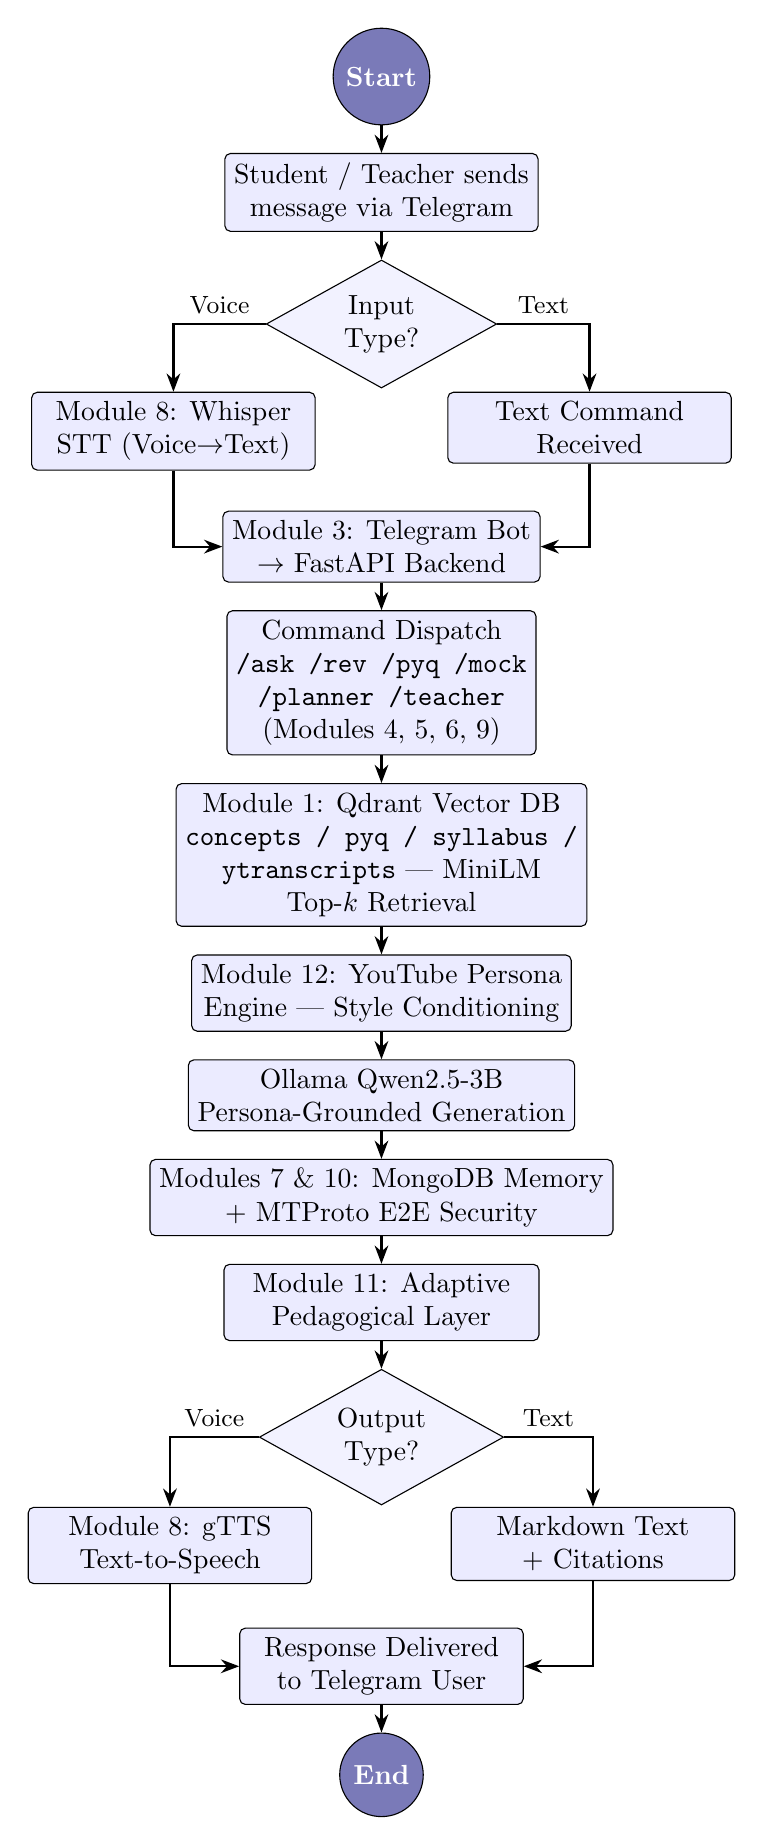
\begin{tikzpicture}[node distance=0.35cm and 0.35cm]
\node[term]  (start)   {Start};
\node[proc,  below=of start]  (send)
      {Student / Teacher sends\\message via Telegram};
\node[dec,   below=of send]   (intype)  {Input\\Type?};
\node[proc,  below left=0.45cm and 0.1cm of intype]  (whisper)
      {Module 8: Whisper\\STT (Voice$\to$Text)};
\node[proc,  below right=0.45cm and 0.1cm of intype] (textrcv)
      {Text Command\\Received};
\node[proc,  below=1.55cm of intype] (fastapi)
      {Module 3: Telegram Bot\\$\to$ FastAPI Backend};
\node[proc,  below=of fastapi] (dispatch)
      {Command Dispatch\\\texttt{/ask /rev /pyq /mock}\\\texttt{/planner /teacher}\\(Modules 4, 5, 6, 9)};
\node[procW, below=of dispatch] (datapipe)
      {Module 1: Qdrant Vector DB\\\texttt{concepts / pyq / syllabus /}\\\texttt{ytranscripts} --- MiniLM\\Top-$k$ Retrieval};
\node[procW, below=of datapipe] (persona)
      {Module 12: YouTube Persona\\Engine --- Style Conditioning};
\node[procW, below=of persona]  (llm)
      {Ollama Qwen2.5-3B\\Persona-Grounded Generation};
\node[procW, below=of llm]      (memsec)
      {Modules 7 \& 10: MongoDB Memory\\+ MTProto E2E Security};
\node[procW, below=of memsec]   (adapt)
      {Module 11: Adaptive\\Pedagogical Layer};
\node[dec,   below=of adapt]     (outtype) {Output\\Type?};
\node[proc,  below left=0.45cm and 0.1cm of outtype]  (gtts)
      {Module 8: gTTS\\Text-to-Speech};
\node[proc,  below right=0.45cm and 0.1cm of outtype] (mdtext)
      {Markdown Text\\+ Citations};
\node[proc,  below=1.55cm of outtype] (deliver)
      {Response Delivered\\to Telegram User};
\node[term,  below=of deliver] (endnode) {End};
\draw[arr] (start)   -- (send);
\draw[arr] (send)    -- (intype);
\draw[arr] (intype)  -| node[near start,above,font=\small]{Voice} (whisper);
\draw[arr] (intype)  -| node[near start,above,font=\small]{Text}  (textrcv);
\draw[arr] (whisper) |- (fastapi);
\draw[arr] (textrcv) |- (fastapi);
\draw[arr] (fastapi) -- (dispatch);
\draw[arr] (dispatch)-- (datapipe);
\draw[arr] (datapipe)-- (persona);
\draw[arr] (persona) -- (llm);
\draw[arr] (llm)     -- (memsec);
\draw[arr] (memsec)  -- (adapt);
\draw[arr] (adapt)   -- (outtype);
\draw[arr] (outtype) -| node[near start,above,font=\small]{Voice} (gtts);
\draw[arr] (outtype) -| node[near start,above,font=\small]{Text}  (mdtext);
\draw[arr] (gtts)    |- (deliver);
\draw[arr] (mdtext)  |- (deliver);
\draw[arr] (deliver) -- (endnode);
\end{tikzpicture}%
}
\caption{StudyMate end-to-end system flowchart. Voice and text inputs
route through FastAPI to the command dispatcher, then traverse the
shared retrieval pipeline augmented by the YouTube Persona Engine
(Module~12), the adaptive pedagogical layer, and encrypted delivery
before reaching the Telegram user.}
\label{fig:flowchart}
\end{figure}
\subsection{Module 1 --- Data Pipeline and Vector Store}
The knowledge layer rests on four Qdrant collections.
\texttt{edu\_concepts} keeps faculty lecture notes and textbook
passages; \texttt{edu\_pyq} holds five years of PYQ papers;
\texttt{edu\_syllabus} stores the official semester-wise syllabus PDFs;
and \texttt{edu\_ytranscripts} carries timestamped segments of YouTube
lecture transcripts tied to registered educator profiles. Following
Koutsiaki et al.~\cite{koutsiaki2025}, we chunk on paragraph
boundaries using \texttt{RecursiveCharacterTextSplitter} at 500 tokens
with 50-token overlap. Each chunk is encoded by
\texttt{all-MiniLM-L6-v2}~\cite{teixeira2025} and written to Qdrant's
HNSW index with payload metadata for source type, educator identifier,
video URL, and timestamp. Curating clean source data up front matters
as much as the model itself, a point stressed in data-collection
practice for machine learning~\cite{roh2021}.
\subsection{Module 2 --- FastAPI Backend and Command Router}
Each webhook message is assigned to one of eight routes: \texttt{/ask}
for open questions, \texttt{/rev} for structured revision, \texttt{/pyq}
for trend analysis, \texttt{/mock} for practice papers, \texttt{/planner}
for scheduling, \texttt{/teacher} for the dashboard, \texttt{/persona}
to register or switch the active educator, and \texttt{/voice} to
toggle audio. LangChain handles prompt assembly, chain execution, and
output formatting the same way across every route.
\subsection{Module 3 --- Telegram Bot Interface}
This module is the system's single point of contact with the student.
Built on \texttt{python-telegram-bot} v20+, it registers a webhook with
Telegram's Bot API and receives every incoming update---text messages,
voice notes, and slash commands---as soon as it arrives, with no
polling delay. Each update is parsed for its Telegram chat ID and user
ID, which are immediately SHA-256-hashed per the Module~10 security
policy before anything is written to storage. The module classifies
the payload by input type: voice notes are forwarded to Module~8 for
Whisper transcription before further processing, while text is passed
through unchanged. Once normalised to text, the message is handed to
Module~2's command router for dispatch. On the way out, the module also
handles Telegram-specific delivery concerns---chunking long Markdown
replies to stay under Telegram's message-length limit, attaching
inline citation links, and returning synthesised voice replies as
OGG/MP3 attachments when Module~8 produces them. Group-chat and
one-to-one contexts are both supported, with per-chat session state
kept isolated so a group deployment cannot leak one student's dialogue
history to another.
\subsection{Module 4 --- PYQ Analysis Engine}
Given a subject code and semester, this module pulls every matching
question from \texttt{edu\_pyq} and runs TF-IDF over five years of
papers to rank topics by recurrence. It also computes how the marks
break down---how many short, mid, and long questions each module has
historically produced---and returns a structured trend report inside
Telegram. None of the systems in Section~II offer this.
\subsection{Module 5 --- Mock Paper Generator}
University papers follow a three-tier shape: short recall items,
mid-length application items, and long evaluation tasks with internal
choice. Using Bloom's Taxonomy~\cite{bloom1984}, the generator places
recall and comprehension at the lowest tier, application and analysis
in the middle, and evaluation or synthesis at the top, calibrating the
mix to the registered subject's historical pattern.
\subsection{Module 6 --- Personalised Study Planner}
The planner reads three inputs: exam dates lifted from the student's
conversation, per-topic score vectors in MongoDB, and module coverage
from \texttt{edu\_syllabus}. Weaker topics get more days, and the plan
is laid out so nothing lands on the final day. After each mock, scores
update and the allocation is recomputed.
\subsection{Module 7 --- Dialogue Tracker (MongoDB)}
Module~7 keeps a per-user record: a SHA-256-hashed identifier, the ten
most recent turns, per-topic scores, weak-topic tags, timestamps,
language preference, and the active educator persona. This context is
prepended to every prompt, giving the coherent multi-turn dialogue that
stateless chatbots cannot.
\subsection{Module 8 --- Voice I/O (Whisper STT + gTTS)}
Telegram voice notes arrive as OGG files and are transcribed by the
Whisper base model, which covers many languages. We expect voice input
to matter most for learners typing non-Latin scripts on phones, where
the keyboard itself is a barrier. For output, gTTS renders the reply to
MP3 and returns it as a voice message, with the locale chosen from the
detected input language.
\subsection{Module 9 --- Teacher Analytics Dashboard}
A Streamlit dashboard shows live class metrics: topic confusion
heatmaps, quiz-score distributions, the week's most-queried concepts,
syllabus coverage, and a panel for which YouTube personas students
activate most. Faculty upload supplementary material or register new
educator URLs here, and the pipeline indexes them without redeployment.
\subsection{Module 10 --- Security Layer}
Transport rides on Telegram's MTProto. At the application layer,
identifiers are SHA-256-hashed, stored content is AES-256-encrypted,
and session-scoped retention keeps personally identifiable data from
outliving the session. Transcript data gets the same treatment---no raw
transcript text is ever logged against a student identifier.
\subsection{Module 11 --- Adaptive Pedagogical Response Layer}
This layer shapes the answer to the learner. It reads recent topic
scores, how often clarifications were requested, preferred language,
and history, then picks a strategy: a concise summary, a step-by-step
breakdown, an analogy, a worked example, or guided Socratic questioning.
The reply stays supportive and grounded strictly in retrieved evidence.
\subsection{Module 12 --- YouTube Transcript Persona Engine}
This is the primary novel contribution.

\textbf{Motivation.} Students routinely say a concept clicks when it is
explained in the voice of a YouTube educator they already follow---not
because the facts change, but because the phrasing, analogies, and
pacing feel familiar. No prior educational RAG system exploits this.

\textbf{Transcript Ingestion.} When someone runs
\texttt{/persona register <url>}, the system calls the YouTube Data API
for the captions or community transcript, splits it into 300-token
windows with 50-token overlap, encodes them with
\texttt{all-MiniLM-L6-v2}, and stores them in \texttt{edu\_ytranscripts}
with educator name, video title, subject tag, and timestamp range.
Multiple videos from one educator roll up into a single profile.

\textbf{Style Fingerprinting.} Before the first reply under a persona,
the system samples thirty transcript passages spread across the
educator's corpus and passes them through a lightweight style-analysis
prompt that produces a persona descriptor---a short structured profile
of sentence length, analogy use, transition phrases, vocabulary
complexity, and whether the educator leans Socratic or declarative.
The descriptor is cached in MongoDB and refreshed only when new videos
arrive.

\textbf{Persona-Grounded Generation.} At inference, retrieval fetches
the top-$k$=3 transcript passages for the active persona alongside the
usual top-$k$=5 from \texttt{edu\_concepts} and \texttt{edu\_syllabus}.
The system prompt is prefixed with the cached descriptor and the
retrieved excerpts, and Qwen2.5-3B is told to deliver the
factual answer---grounded in the institutional corpus---in the style
the descriptor specifies. With no active persona, control falls back to
the standard adaptive layer. The style-transfer idea itself follows
prior style-conditioned generation work~\cite{li2023}, adapted here to
a grounded setting.

\textbf{Persona Style Consistency (PSC).} Judging whether an answer
truly reflects an educator's style needs a metric beyond RAGAS. PSC
shows a separate LLM judge each generated answer next to three genuine
excerpts from the registered educator and three from a neutral
baseline, and asks it to label the answer style-consistent or not. PSC
is the fraction judged consistent; we target PSC $\geq 0.78$, a
threshold pilot observations link to students rating a reply ``sounds
like my lecturer'' above 70\% of the time.

\textbf{Fallback and Safety.} If fewer than five transcript passages
match the query for the active persona, the persona layer is silently
skipped and a standard answer is returned---a guard against
hallucinated style attribution when coverage is thin.

\subsection{Hallucination Detection and Avoidance}
Because a grounded system can still fabricate, we treat hallucination
control as a first-class design concern rather than an afterthought,
and combat it at four points in the pipeline.

First, \emph{retrieval gating}. Every retrieved passage carries a
cosine-similarity score; if the best passage for a query falls below a
tuned threshold, the model is not asked to answer from weak evidence at
all. Instead it returns an explicit ``this is not covered in your
course material'' message and points the student to the relevant
chapter. This converts a likely fabrication into an honest miss.

Second, \emph{grounded prompting with abstention}. Every system prompt
carries a hard instruction to answer only from the retrieved context
and to say so when the context is silent. The persona prefix is
deliberately scoped to \emph{style only}; it may change phrasing but is
forbidden from adding facts, which prevents the persona layer from
becoming a second, ungrounded source.

Third, \emph{automated faithfulness screening}. During evaluation the
RAGAS Faithfulness score (Section~VI-A) flags any answer whose claims
cannot be traced to retrieved context. Answers below the $0.85$
threshold are logged for review, giving a measurable, repeatable audit
of hallucination rate rather than an anecdotal one.

Fourth, \emph{human-in-the-loop and citation}. Text replies carry
inline citations to the source passage so students and faculty can
verify them, and the teacher dashboard surfaces low-faithfulness
answers for correction. Persona coverage below the five-passage floor
disables styling entirely, so the system never invents an educator's
voice it cannot support.
%------------------------------------------------
\section{Implementation Details}
%------------------------------------------------
\subsection{Technology Stack}
Table~\ref{tab:stack} lists the full stack. Adding the persona engine
required only three new pieces---the YouTube Data API v3, a
style-fingerprinting prompt layer, and the \texttt{edu\_ytranscripts}
collection---while everything else stayed as in the base architecture.
\begin{table}[htbp]
\caption{StudyMate Technology Stack}
\label{tab:stack}
\begin{tabular}{ll}
\toprule
\textbf{Component}             & \textbf{Technology} \\
\midrule
Language                       & Python 3.10+ \\
Backend Framework              & FastAPI \\
Orchestration                  & LangChain \\
LLM Runtime                    & Ollama (Qwen2.5-3B; 7B for mock papers) \\
Embedding Model                & all-MiniLM-L6-v2 \\
Vector Database                & Qdrant (self-hosted) \\
Bot Framework                  & python-telegram-bot v20+ \\
Dialogue Memory                & MongoDB Atlas \\
STT                            & Whisper base (OpenAI) \\
TTS                            & gTTS \\
Transcript Ingestion           & YouTube Data API v3 \\
Style Fingerprinting           & LangChain prompt + Qwen2.5-3B \\
Teacher Dashboard              & Streamlit \\
Security                       & MTProto, AES-256, SHA-256 \\
Deployment                     & AWS EC2 t3.medium, Docker \\
Evaluation                     & RAGAS, PSC, TAM ($N{\geq}30$) \\
\bottomrule
\end{tabular}
\end{table}
\subsection{RAG Pipeline}
A response passes through six stages.
\begin{enumerate}
    \item \textbf{Ingestion}: \texttt{PyPDFLoader} loads PDFs and the
          YouTube Data API pulls transcripts; both are chunked with
          \texttt{RecursiveCharacterTextSplitter}
          (500/50 for documents, 300/50 for transcripts).
    \item \textbf{Embedding}: \texttt{all-MiniLM-L6-v2} encodes each
          passage into a 384-dimensional vector~\cite{teixeira2025}.
    \item \textbf{Indexing}: Qdrant stores the vectors in an HNSW index
          with source type, educator identifier, subject code, module
          number, and year as payload.
    \item \textbf{Retrieval}: cosine similarity returns the top-$k$=5
          institutional passages and, if a persona is active, the
          top-$k$=3 transcript passages.
    \item \textbf{Persona Conditioning}: the cached descriptor and
          transcript excerpts are prepended to the system prompt.
    \item \textbf{Generation}: the assembled context, query, and
          persona-conditioned prompt go to Qwen2.5-3B via the local
          Ollama API.
\end{enumerate}
\subsection{Prompt Engineering and Bloom's Integration}
Prompt design adapts the three roles of Lauber et al.~\cite{lauber2025}:
\texttt{/ask} and \texttt{/rev} run a \textit{Learning Instructor} role,
\texttt{/mock} a \textit{Learning Partner}, and \texttt{/planner} a
\textit{Learning Assistant}. Every prompt carries the hard constraint
to admit when retrieved context does not cover a question and to send
the student to their textbook. When a persona is active, the prompt
gains a prefix of the form: \textit{``Answer as [Educator Name] would
explain it, using their typical analogies and phrasing as shown in the
transcript excerpts. The factual content must stay grounded in the
retrieved course material.''} This two-layer prompt---institutional
grounding plus persona style---is the mechanism that keeps answers both
accurate and familiar.
\subsection{User Interface}
The Telegram bot is complemented by a Next.js web workspace that
exposes the same eight tools through a single-page study interface,
letting the implementation be inspected independently of a Telegram
account. Fig.~\ref{fig:ui-ask} shows the default \texttt{/ask} view:
subject, year, and board selectors sit above the question field, with
the YouTube persona selector and live backend health status visible on
first load. Fig.~\ref{fig:ui-guided} and Fig.~\ref{fig:ui-revision}
show the Guided Learning (Socratic) and Revision Notes tools, which
share the same course-selection chrome but swap the input fields and
call-to-action for the task at hand. Fig.~\ref{fig:ui-pyq} shows the
Past Paper Review tool that fronts Module~4's TF-IDF trend engine, and
Fig.~\ref{fig:ui-mock} shows the Practice Paper tool that fronts
Module~5's Bloom's-taxonomy generator, with total marks configurable
before generation. Fig.~\ref{fig:ui-persona} shows the YouTube Transcript
Persona Engine (Module~12) panel used to register an educator's lecture
URL, choose a caption language, and select the active teaching style for
subsequent answers. Fig.~\ref{fig:ui-planner} shows the Study Plan
\& Scores panel that fronts Module~6's exam-date-aware planner.
Fig.~\ref{fig:ui-teacher} shows the Teacher Tools dashboard (Module~9),
gated behind a teacher access key, for reviewing aggregated learning
activity and maintaining the course corpus. All screenshots below show
the interface prior to submission, so no model-generated content is
depicted.

\begin{figure}[!t]
\centering
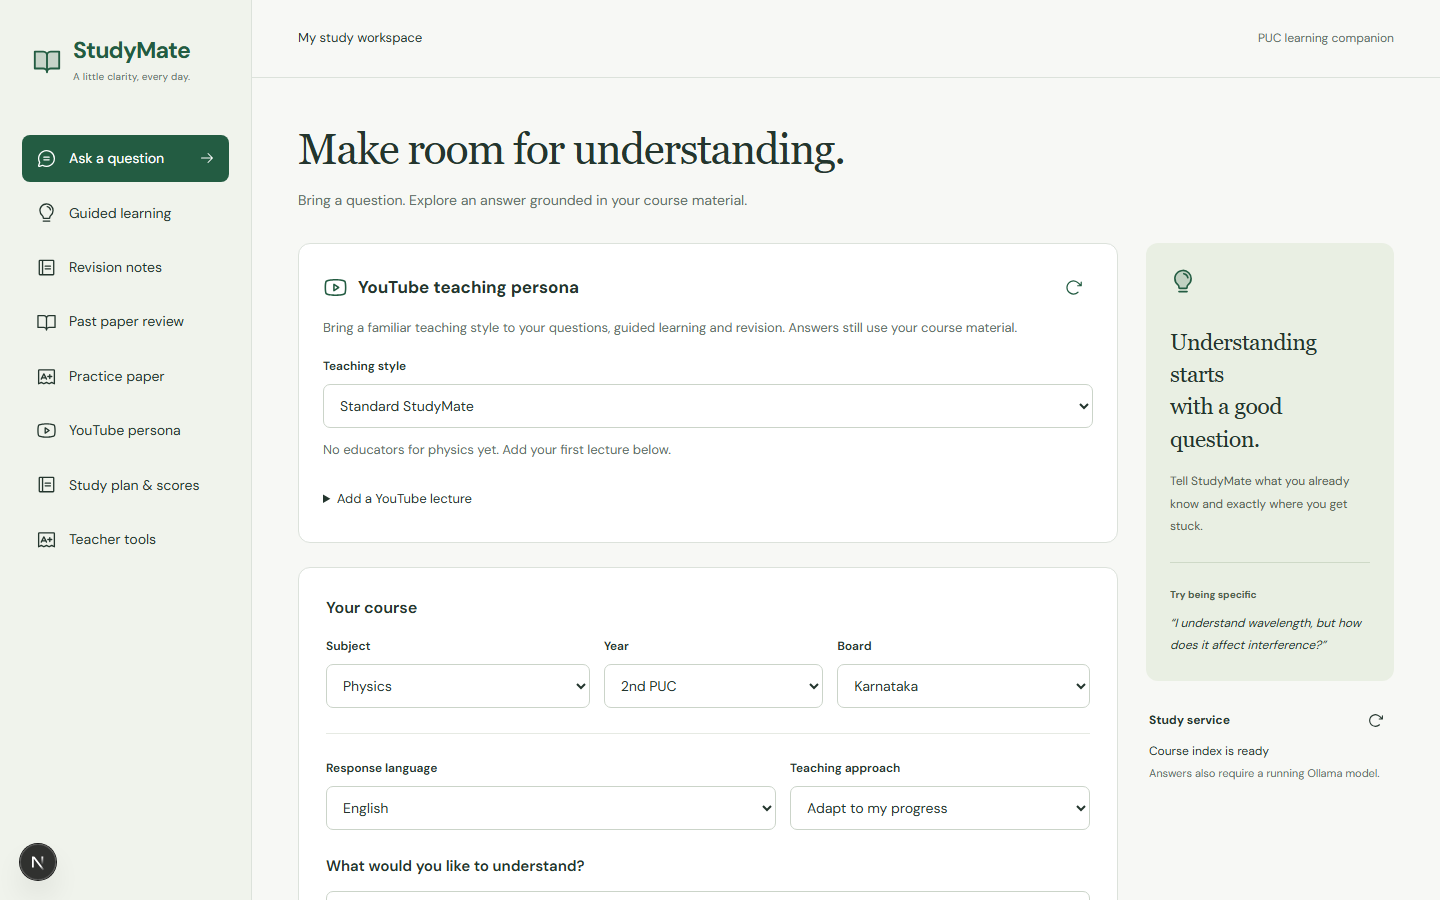
\includegraphics[width=\columnwidth]{figures/01-ask.png}
\caption{Ask a question --- the default study view, with course
selectors, the YouTube persona selector, and live backend status.}
\label{fig:ui-ask}
\end{figure}

\begin{figure}[!t]
\centering
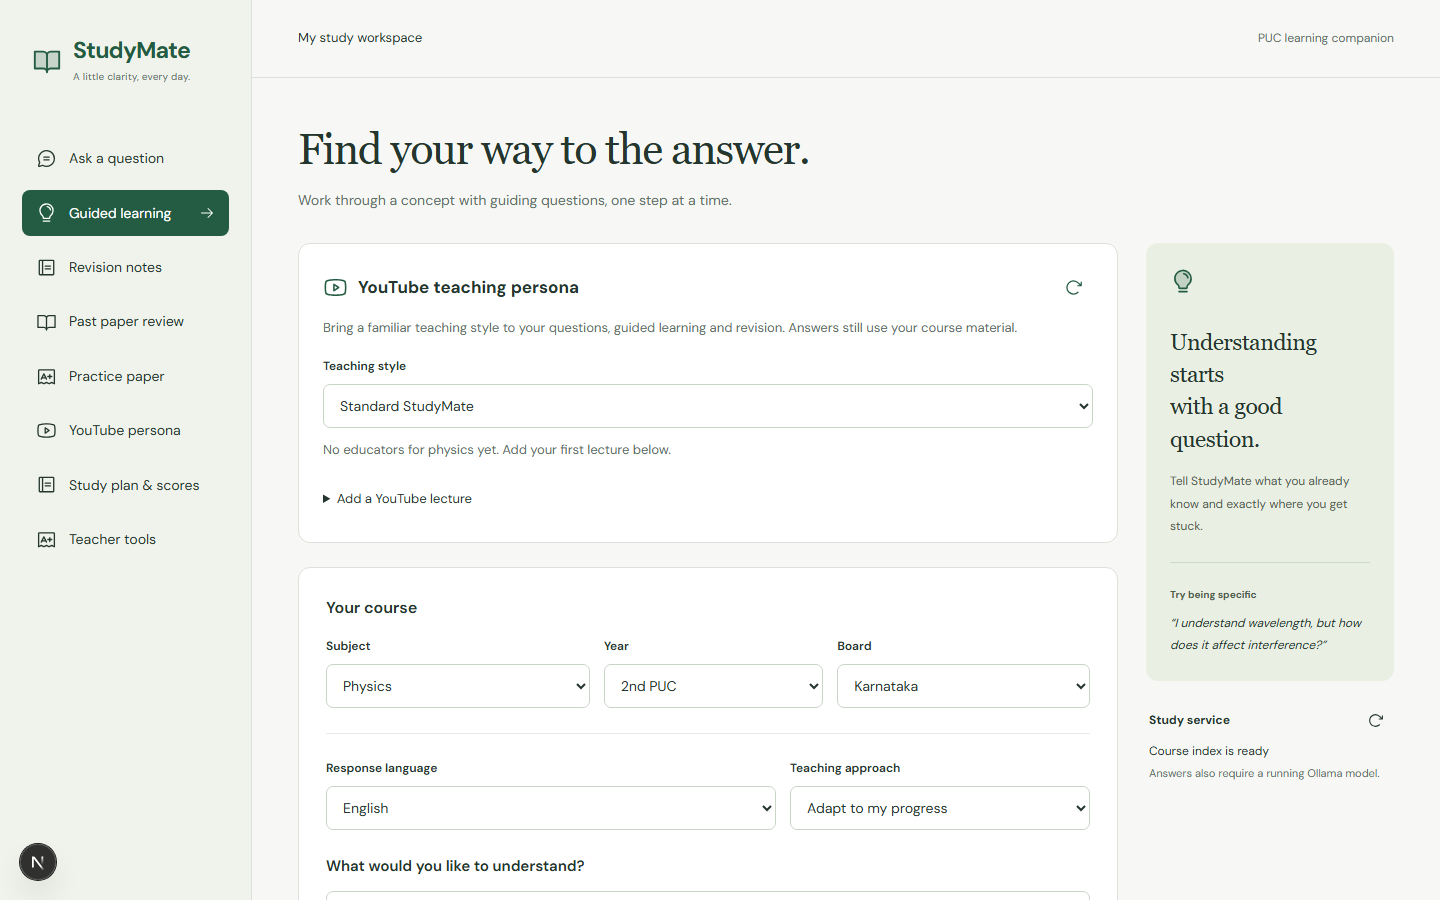
\includegraphics[width=\columnwidth]{figures/02-guided-learning.png}
\caption{Guided learning --- the Socratic tutoring tool (Module~11
adaptive strategy: guiding questions).}
\label{fig:ui-guided}
\end{figure}

\begin{figure}[!t]
\centering
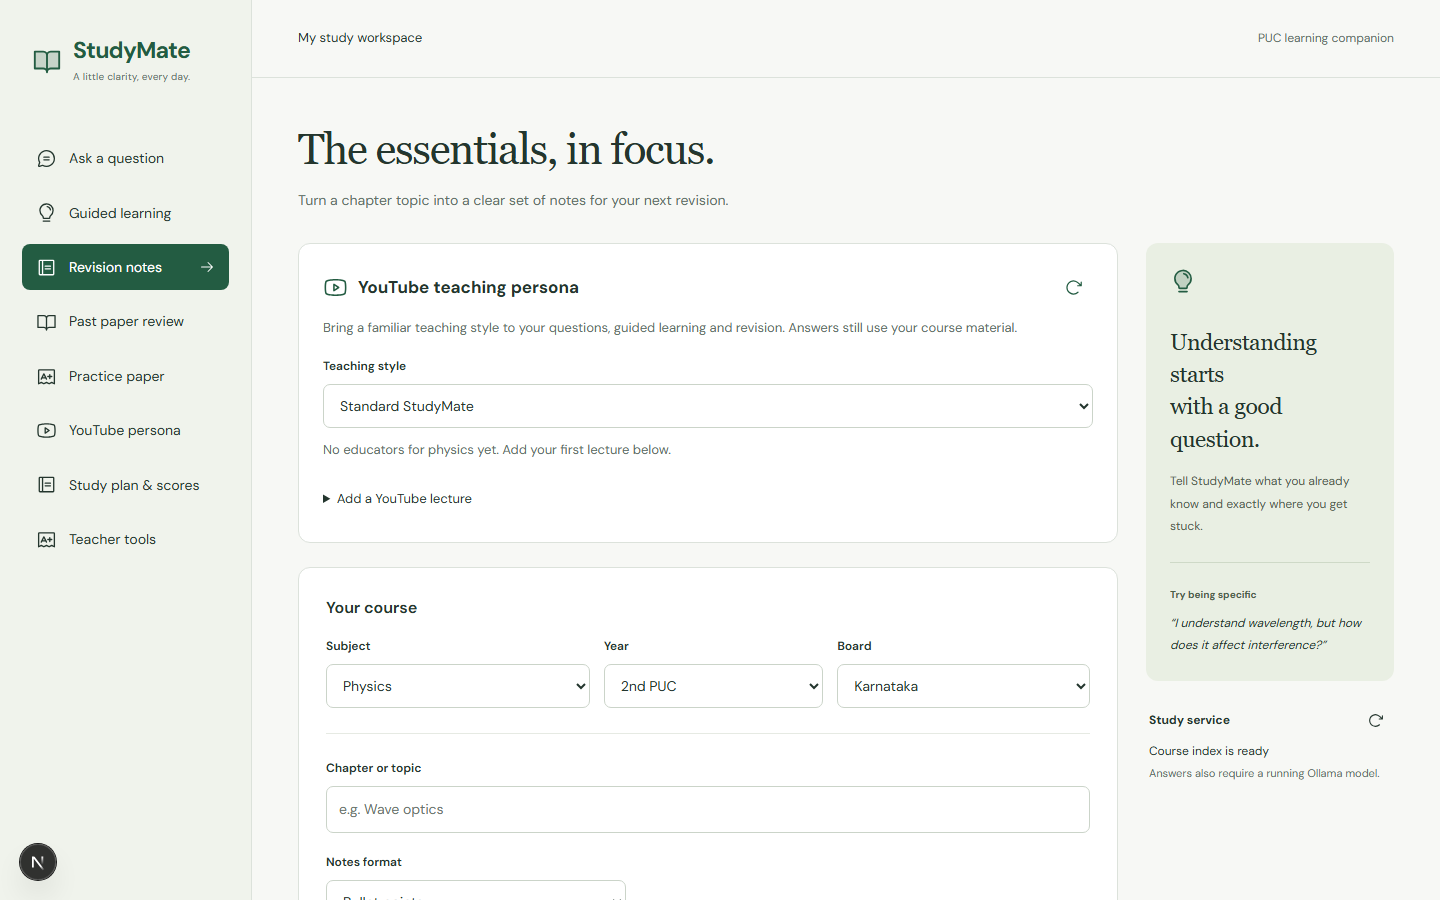
\includegraphics[width=\columnwidth]{figures/03-revision-notes.png}
\caption{Revision notes --- chapter-to-notes tool with selectable notes
format.}
\label{fig:ui-revision}
\end{figure}

\begin{figure}[!t]
\centering
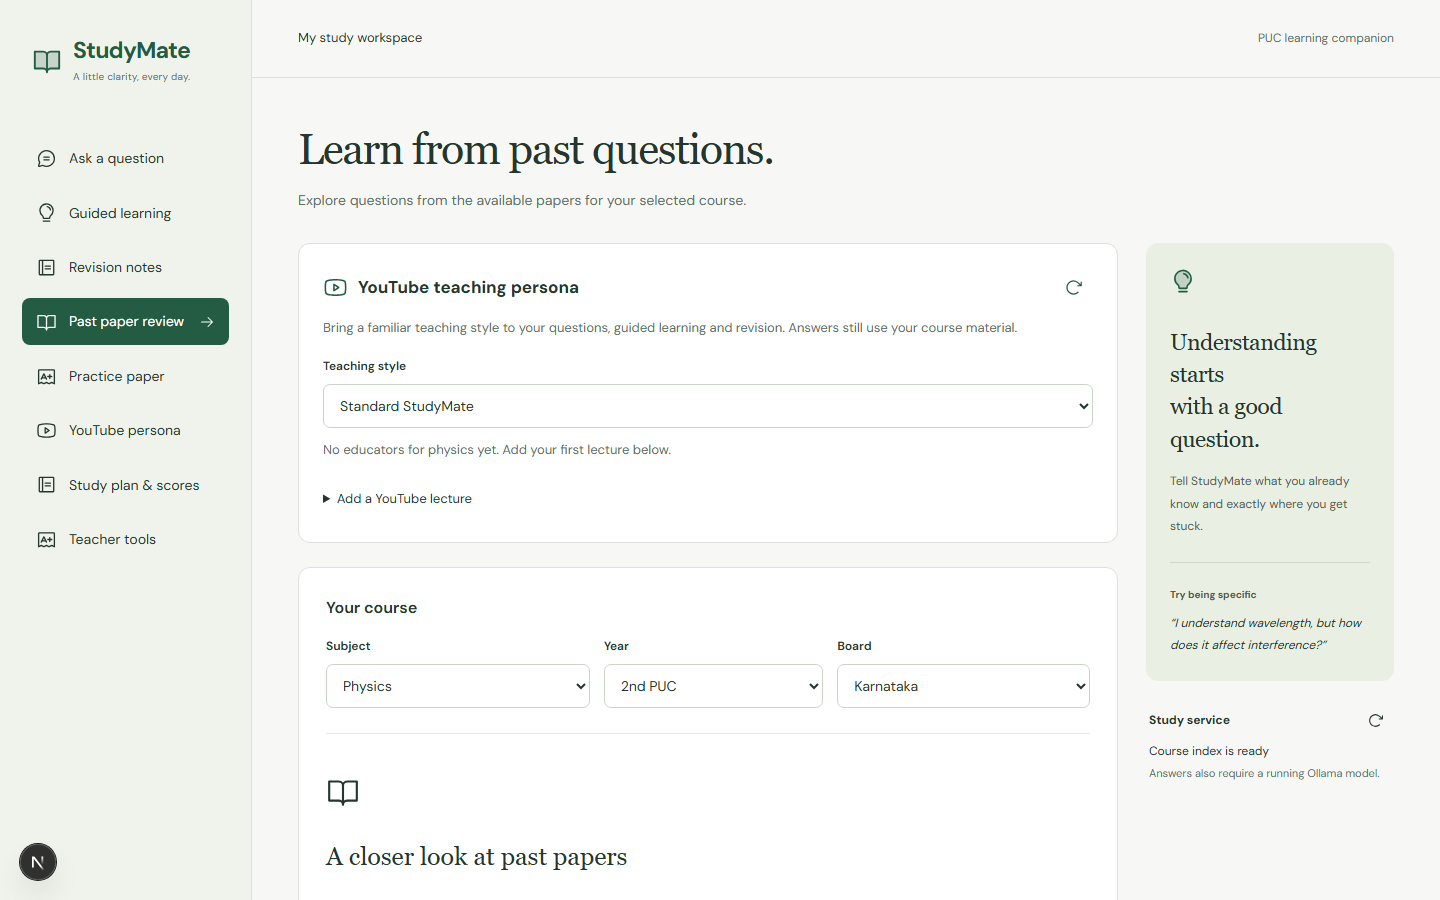
\includegraphics[width=\columnwidth]{figures/04-past-paper-review.png}
\caption{Past paper review --- front end for the PYQ trend engine
(Module~4).}
\label{fig:ui-pyq}
\end{figure}

\begin{figure}[!t]
\centering
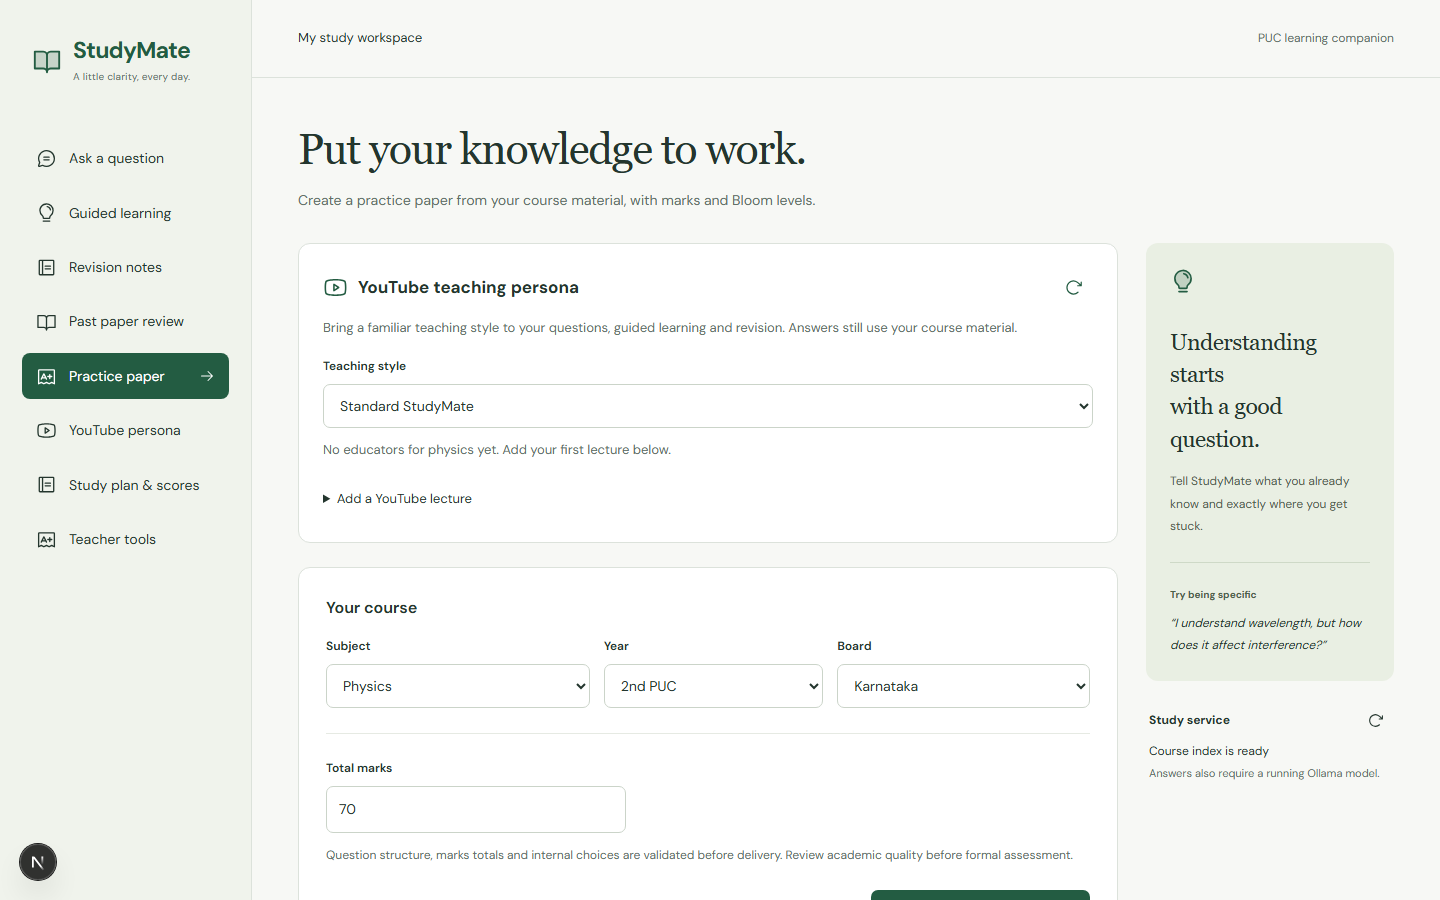
\includegraphics[width=\columnwidth]{figures/05-practice-paper.png}
\caption{Practice paper --- front end for the Bloom's-taxonomy mock
generator (Module~5), with configurable total marks.}
\label{fig:ui-mock}
\end{figure}

\begin{figure}[!t]
\centering
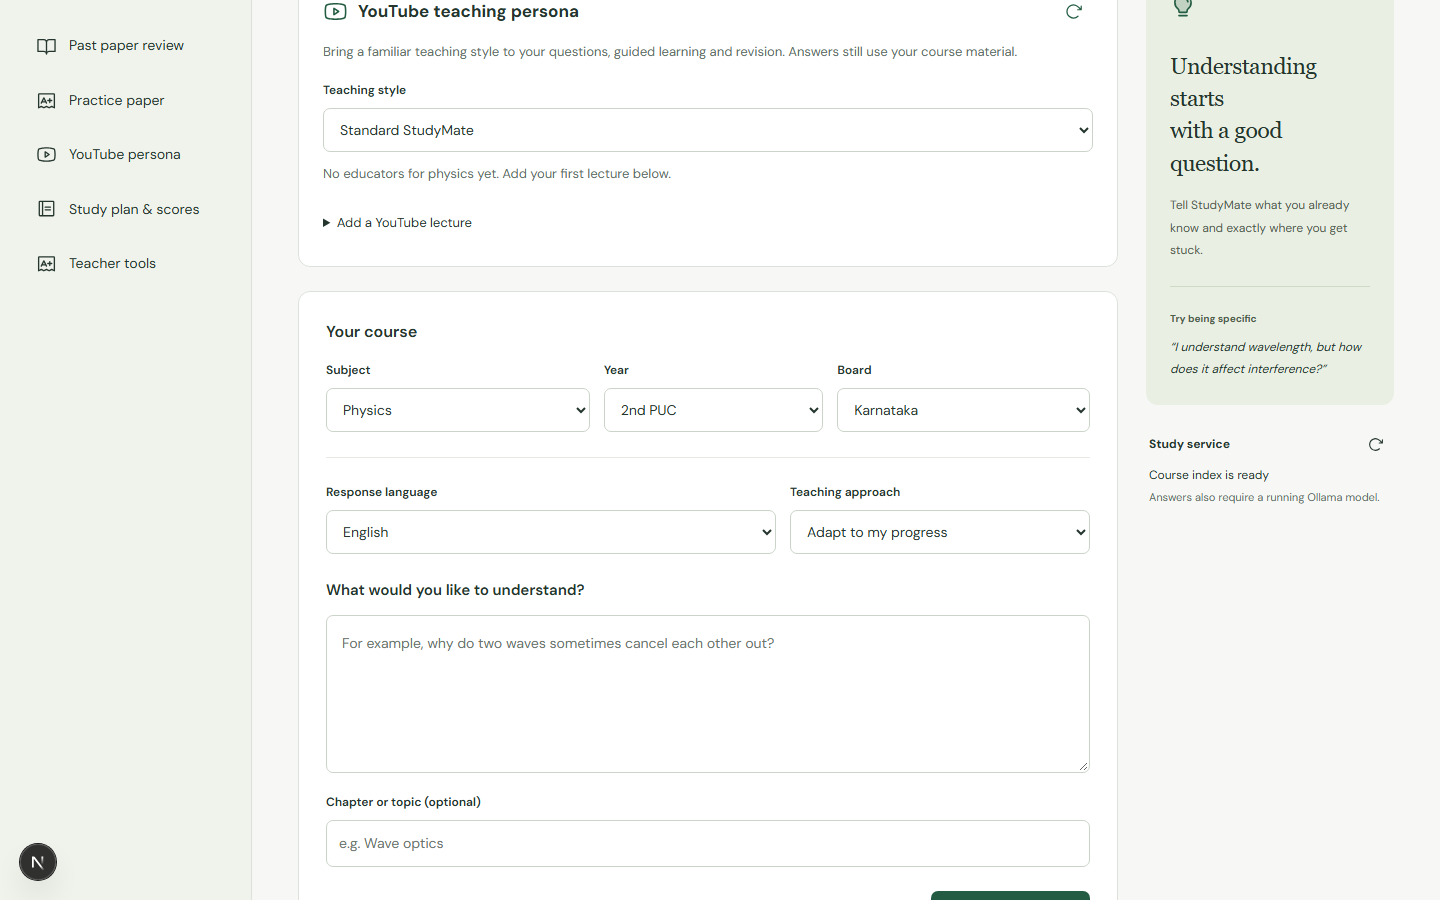
\includegraphics[width=\columnwidth]{figures/06-youtube-persona.png}
\caption{YouTube Transcript Persona Engine panel (Module~12) --- register
an educator's lecture URL and select a teaching style.}
\label{fig:ui-persona}
\end{figure}

\begin{figure}[!t]
\centering
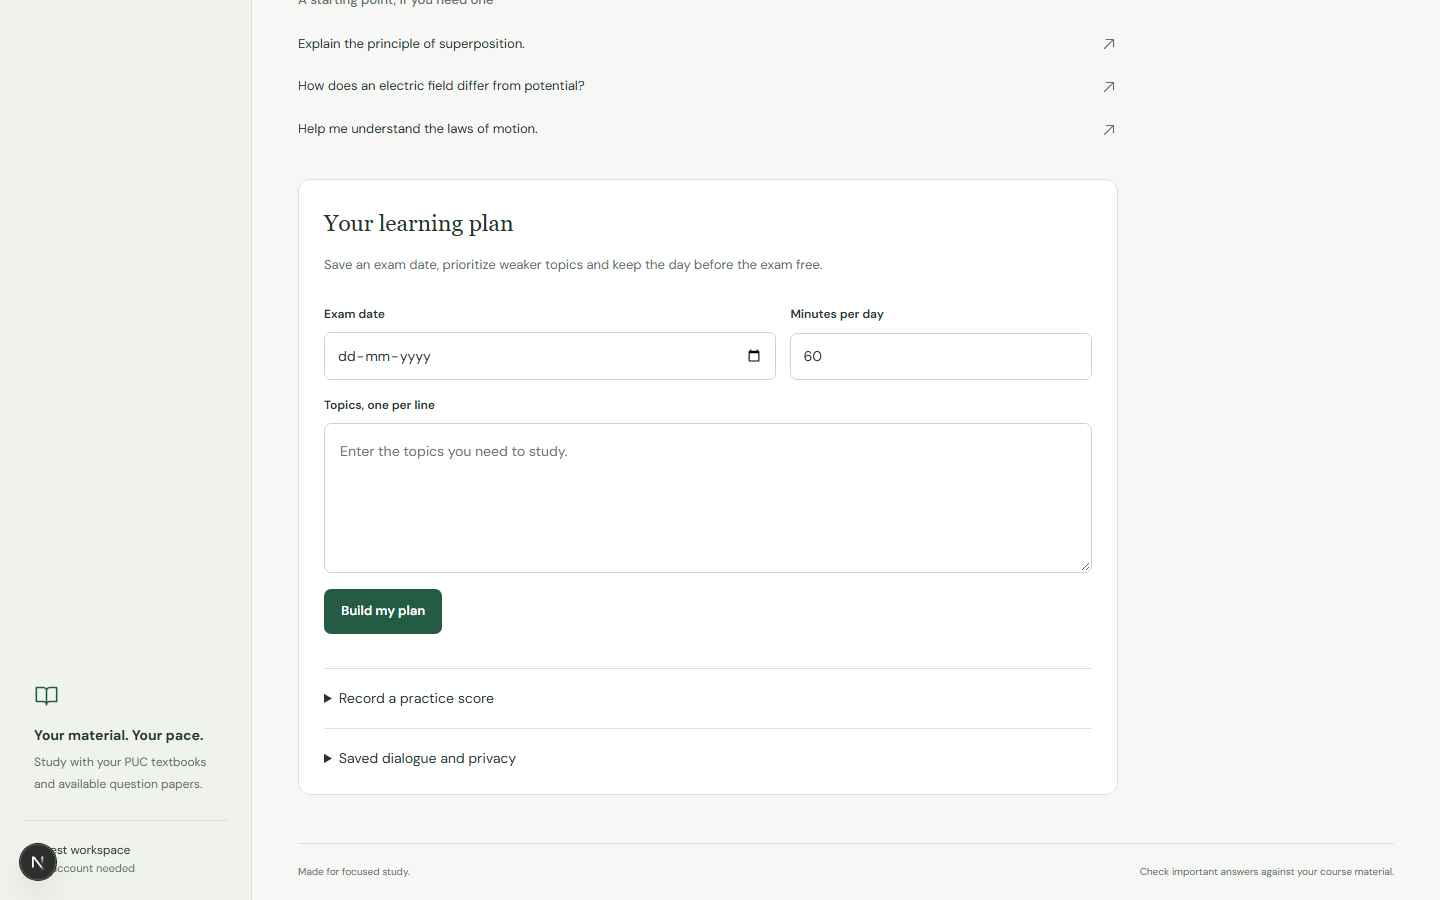
\includegraphics[width=\columnwidth]{figures/07-study-plan.png}
\caption{Study plan \& scores --- front end for the personalised study
planner (Module~6).}
\label{fig:ui-planner}
\end{figure}

\begin{figure}[!t]
\centering
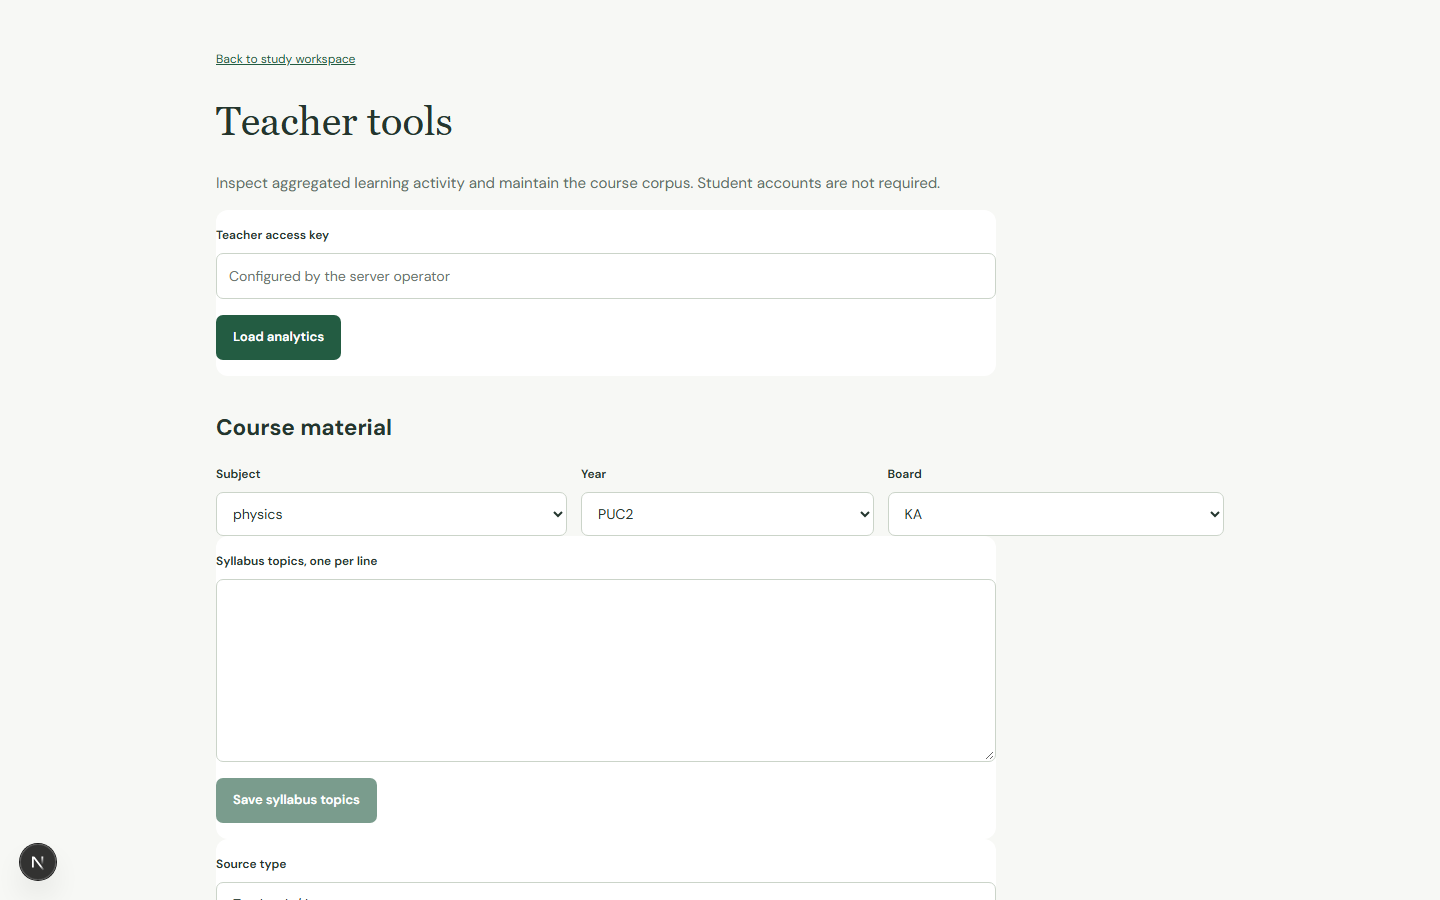
\includegraphics[width=\columnwidth]{figures/08-teacher-tools.png}
\caption{Teacher tools dashboard (Module~9) --- access-key-gated
analytics and course-corpus maintenance.}
\label{fig:ui-teacher}
\end{figure}

\subsection{Working System Output}
The figures in this subsection are live outputs from the deployed
prototype, captured against an index of 7{,}669 chunks built from the
PUC physics, chemistry, mathematics, and biology corpora, with
Qwen2.5-3B served locally through Ollama. Fig.~\ref{fig:r-ask} shows a
grounded answer to a wave-optics question: the explanation carries
inline \texttt{[1]}, \texttt{[2]} markers and a \emph{Retrieved
sources} list naming the textbook file and page for every cited
passage, which is the citation mechanism described in
Section~IV-L. Fig.~\ref{fig:r-guided} and Fig.~\ref{fig:r-revision}
show the Socratic and revision-notes variants of the same pipeline.
Fig.~\ref{fig:r-pyq} shows a real PYQ trend report over 102 extracted
questions, with per-topic recurrence, the years each topic appeared in,
the mark distribution, and an explicit statement of which years in the
five-year window are missing from the supplied archive.
Fig.~\ref{fig:r-mock} shows a generated 70-mark practice paper whose
Bloom levels ascend from \emph{understand} through \emph{apply} and
\emph{evaluate} to \emph{analyze}, and which renders an internal choice
as an \emph{OR} alternative at matching marks, reproducing the
three-tier shape described in Section~IV-D.
Fig.~\ref{fig:r-planner} shows a generated 99-day study plan that
distributes five topics across daily sessions and, as
Section~IV-E specifies, keeps the day before the exam free.

Two qualifications apply to paper generation. Retrieval for this module
must be seeded with actual examination topics: querying the index with
the bare subject name returns title pages and prefaces, which yielded a
paper asking about the textbook's own structure rather than its physics.
Seeding retrieval from the recurring PYQ topics of Module~4 --- the
historical calibration Section~IV-D already calls for --- removed those
items. Separately, this is the one figure not produced by the local
runtime: a 3B model cannot hold a fifteen-question blueprint in valid
JSON, and the 7B model exceeded the practical latency budget on our
host, so the paper in Fig.~\ref{fig:r-mock} was generated with Gemini
2.5 Flash through Vertex AI. Interactive tutoring remains local; we
treat structured paper generation as the component whose model choice
is dictated by output validity rather than by privacy alone.

Fig.~\ref{fig:r-persona} shows the Module~12 style fingerprint for a
registered Class~11 physics lecture. The profile correctly identifies
Hindi--English code-switching, the speaker's Hindi discourse markers,
the mix of English technical vocabulary with Hindi fillers, and a
step-by-step questioning approach --- evidence that the fingerprinting
stage recovers observable stylistic structure rather than course
facts. Two caveats apply to this figure and are stated here rather than
in the caption alone. First, the lecture's captions run to 219{,}041
embedding tokens against the engine's 100{,}000-token ceiling, so the
opening excerpt was registered through the supported paste-transcript
path and is labelled \emph{user-supplied transcript} in the interface.
Second, style conditioning did not subsequently fire for this educator:
with the English-trained \texttt{all-MiniLM-L6-v2} encoder, an English
question retrieves the English course corpus but matches fewer than
five Hindi transcript passages, so the five-passage floor of
Section~IV-K correctly suppressed styling, while a Hindi question fails
the course-evidence gate instead. Cross-lingual persona conditioning
therefore requires a multilingual encoder; we record this as a
limitation of the present configuration rather than of the design, and
revisit it in Section~VI-E.

\begin{figure}[!t]
\centering
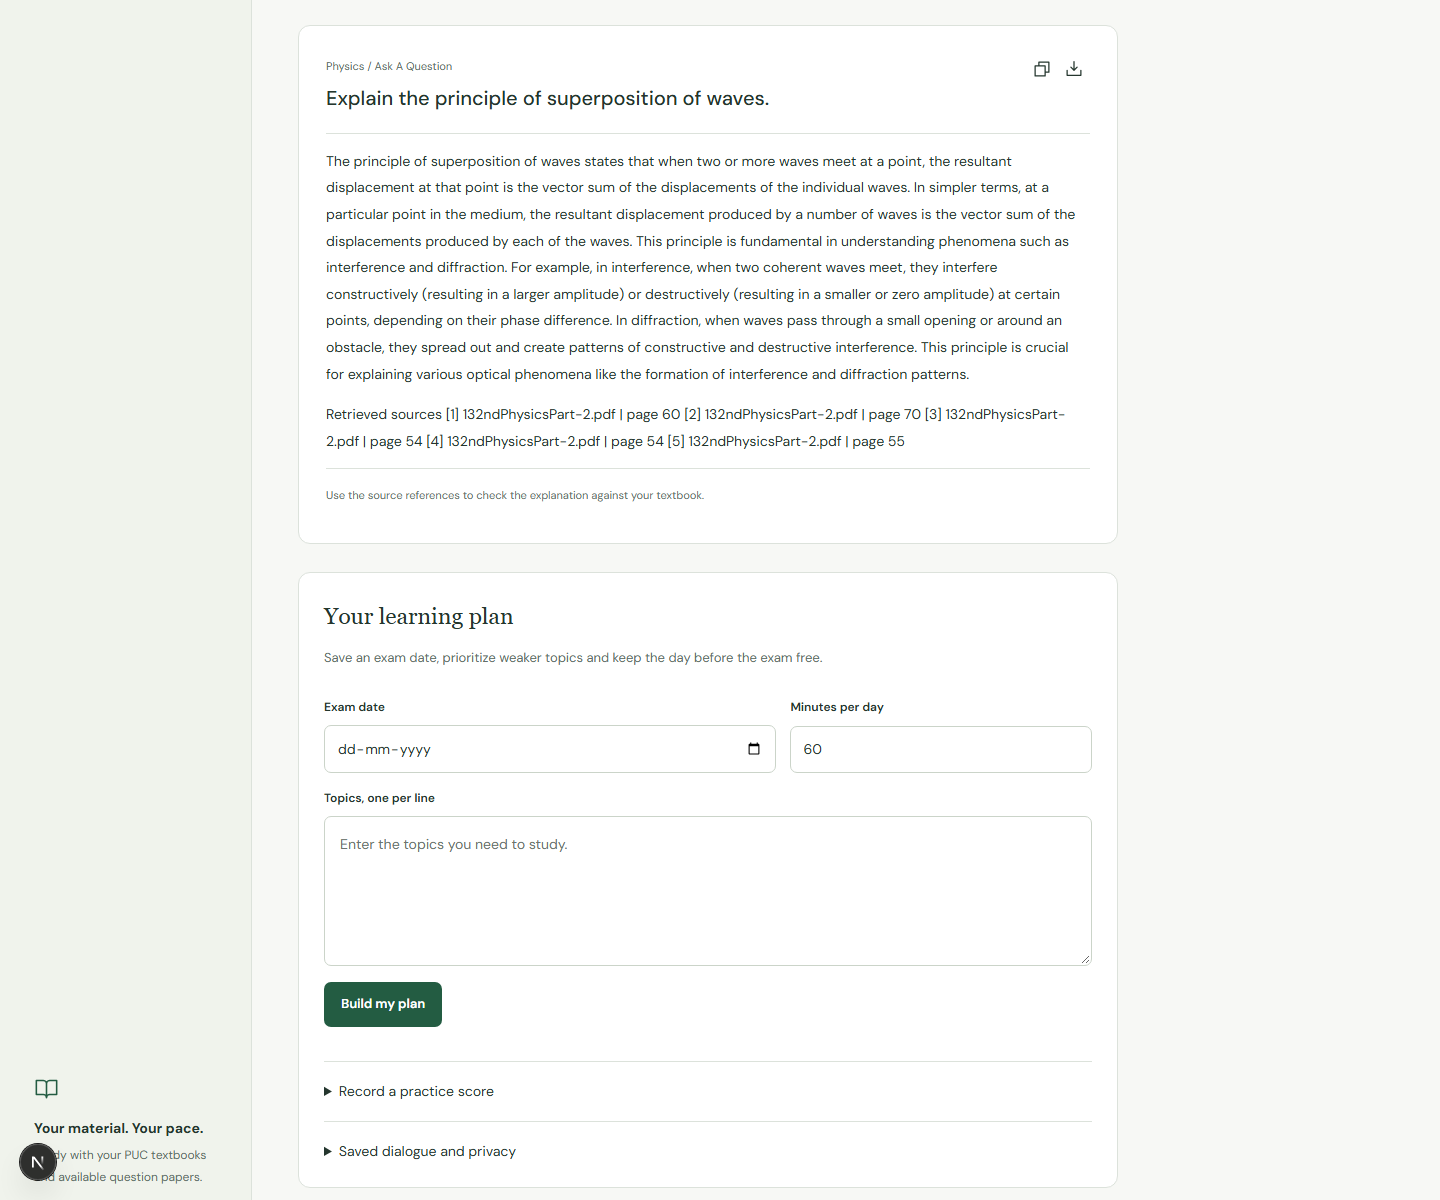
\includegraphics[width=\columnwidth]{figures/r01-ask-result.png}
\caption{Grounded answer with inline citations resolving to textbook
file and page numbers.}
\label{fig:r-ask}
\end{figure}

\begin{figure}[!t]
\centering
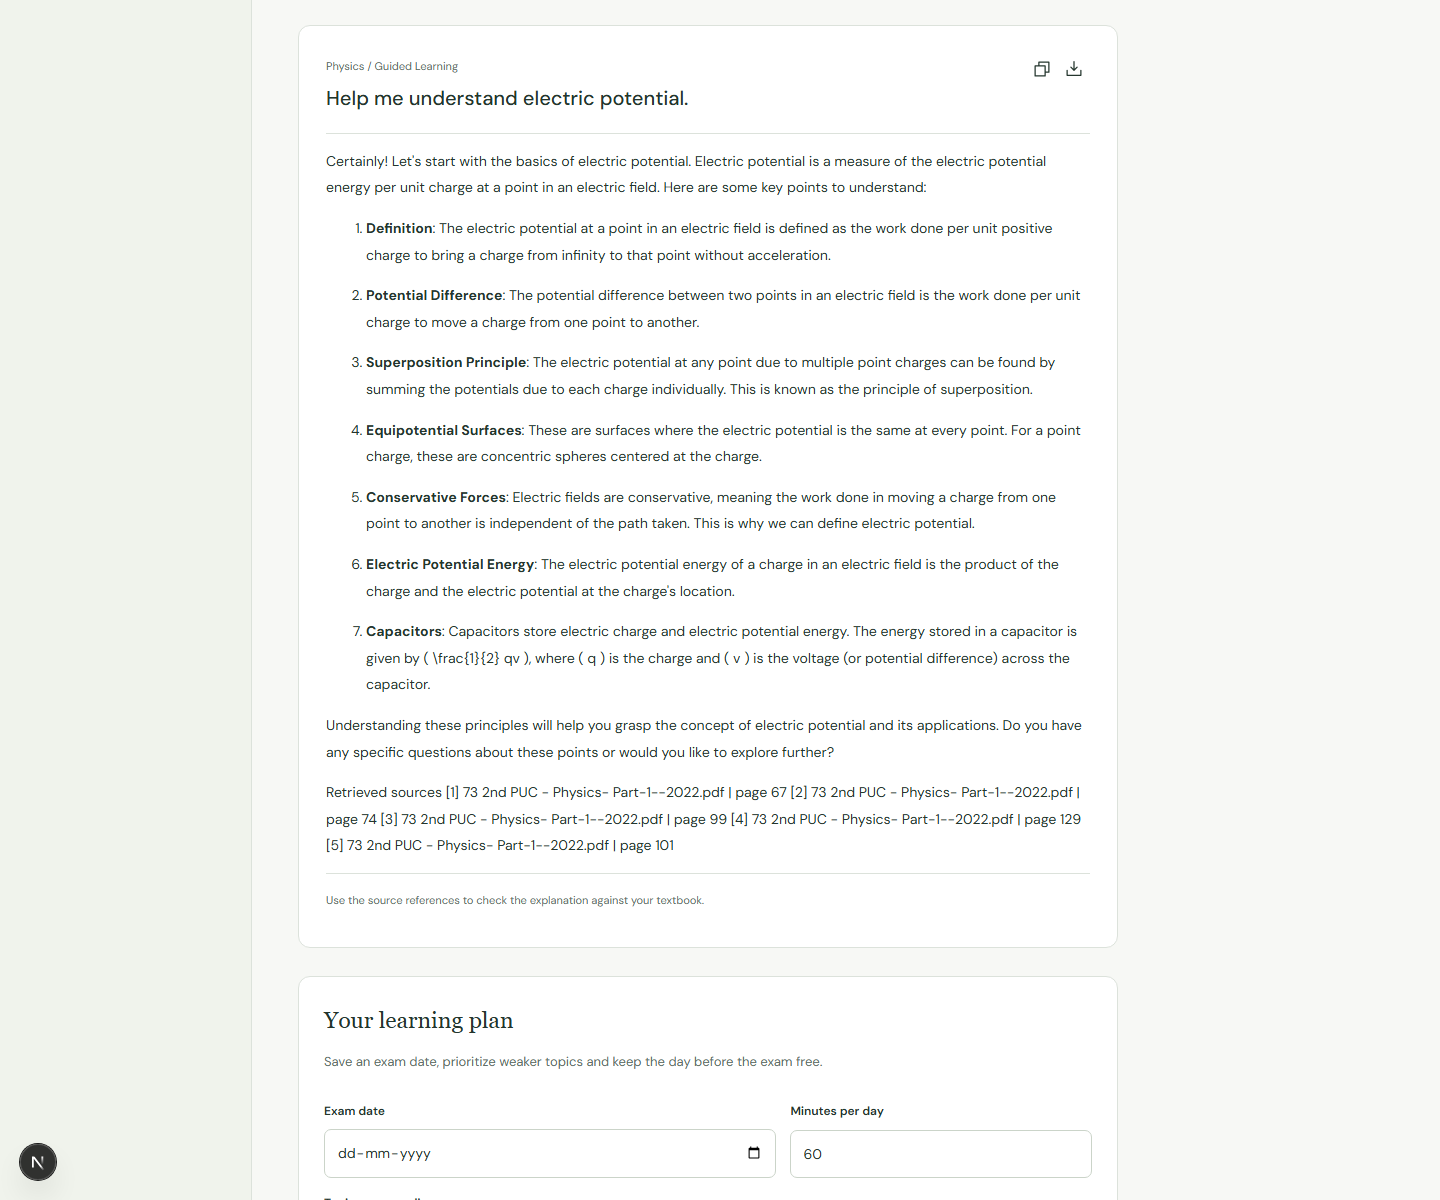
\includegraphics[width=\columnwidth]{figures/r02-guided-result.png}
\caption{Guided learning output --- the Socratic role of
Section~V-C.}
\label{fig:r-guided}
\end{figure}

\begin{figure}[!t]
\centering
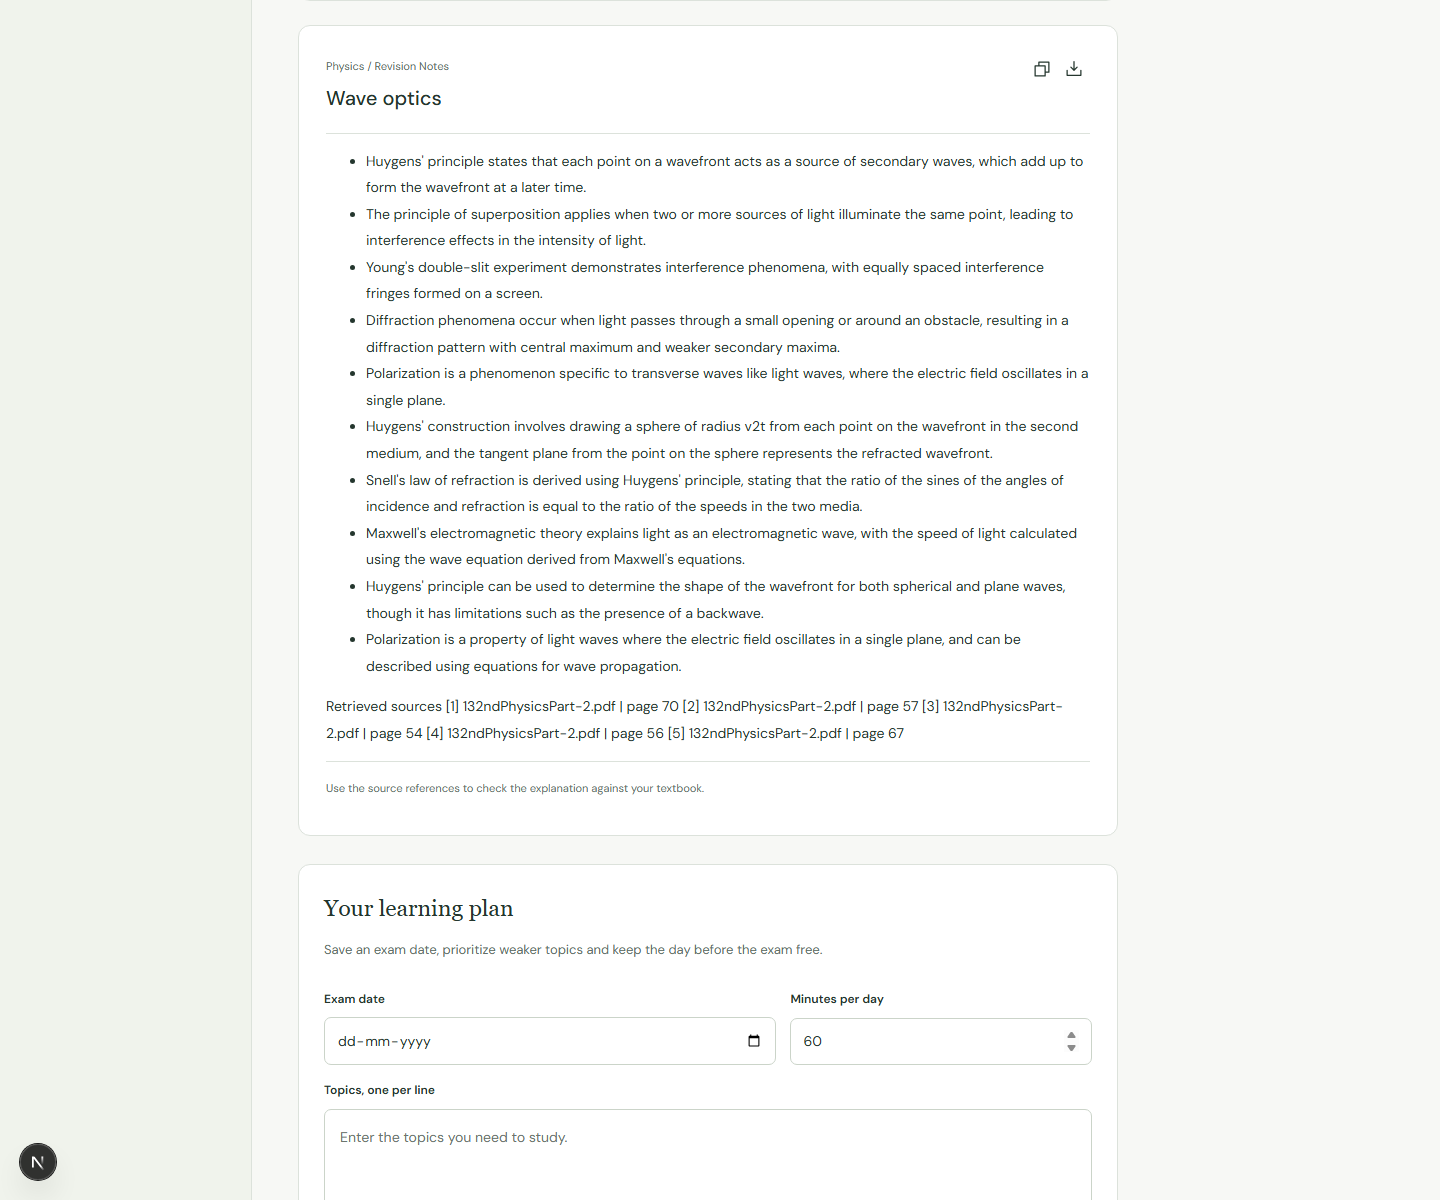
\includegraphics[width=\columnwidth]{figures/r03-revision-result.png}
\caption{Generated revision notes for a requested chapter topic.}
\label{fig:r-revision}
\end{figure}

\begin{figure}[!t]
\centering
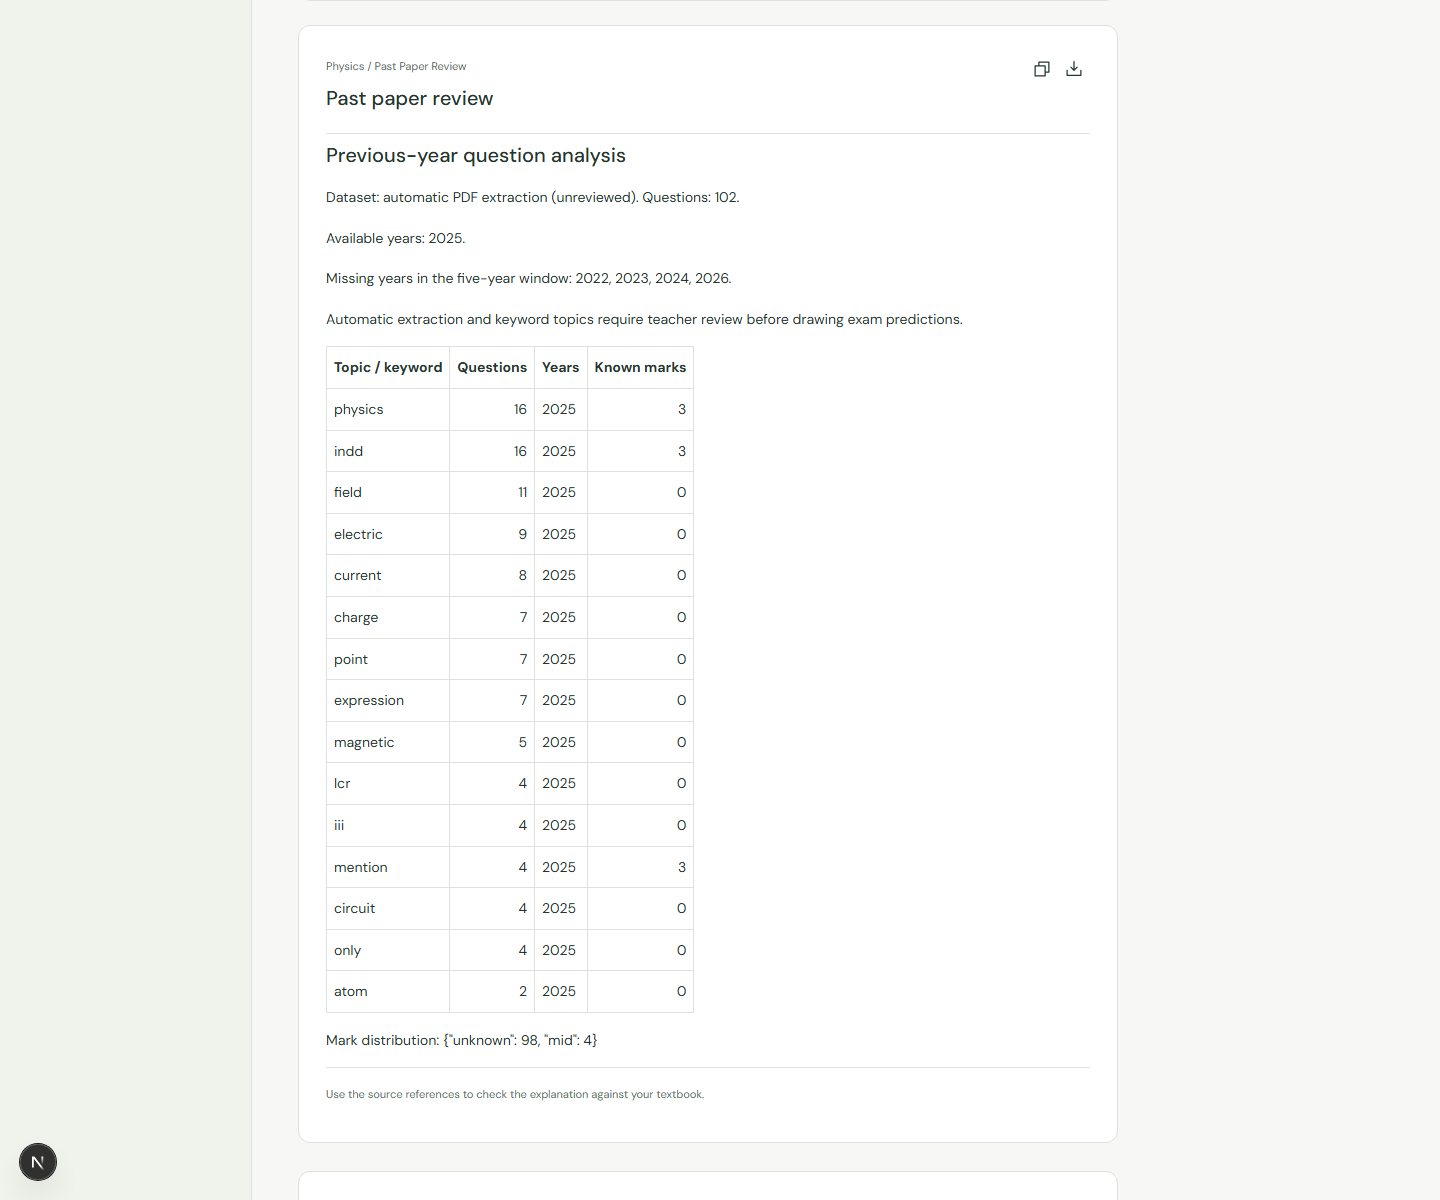
\includegraphics[width=\columnwidth]{figures/r04-pyq-result.png}
\caption{PYQ trend report (Module~4) over 102 extracted questions:
topic recurrence, mark distribution, and missing years reported
explicitly.}
\label{fig:r-pyq}
\end{figure}

\begin{figure}[!t]
\centering
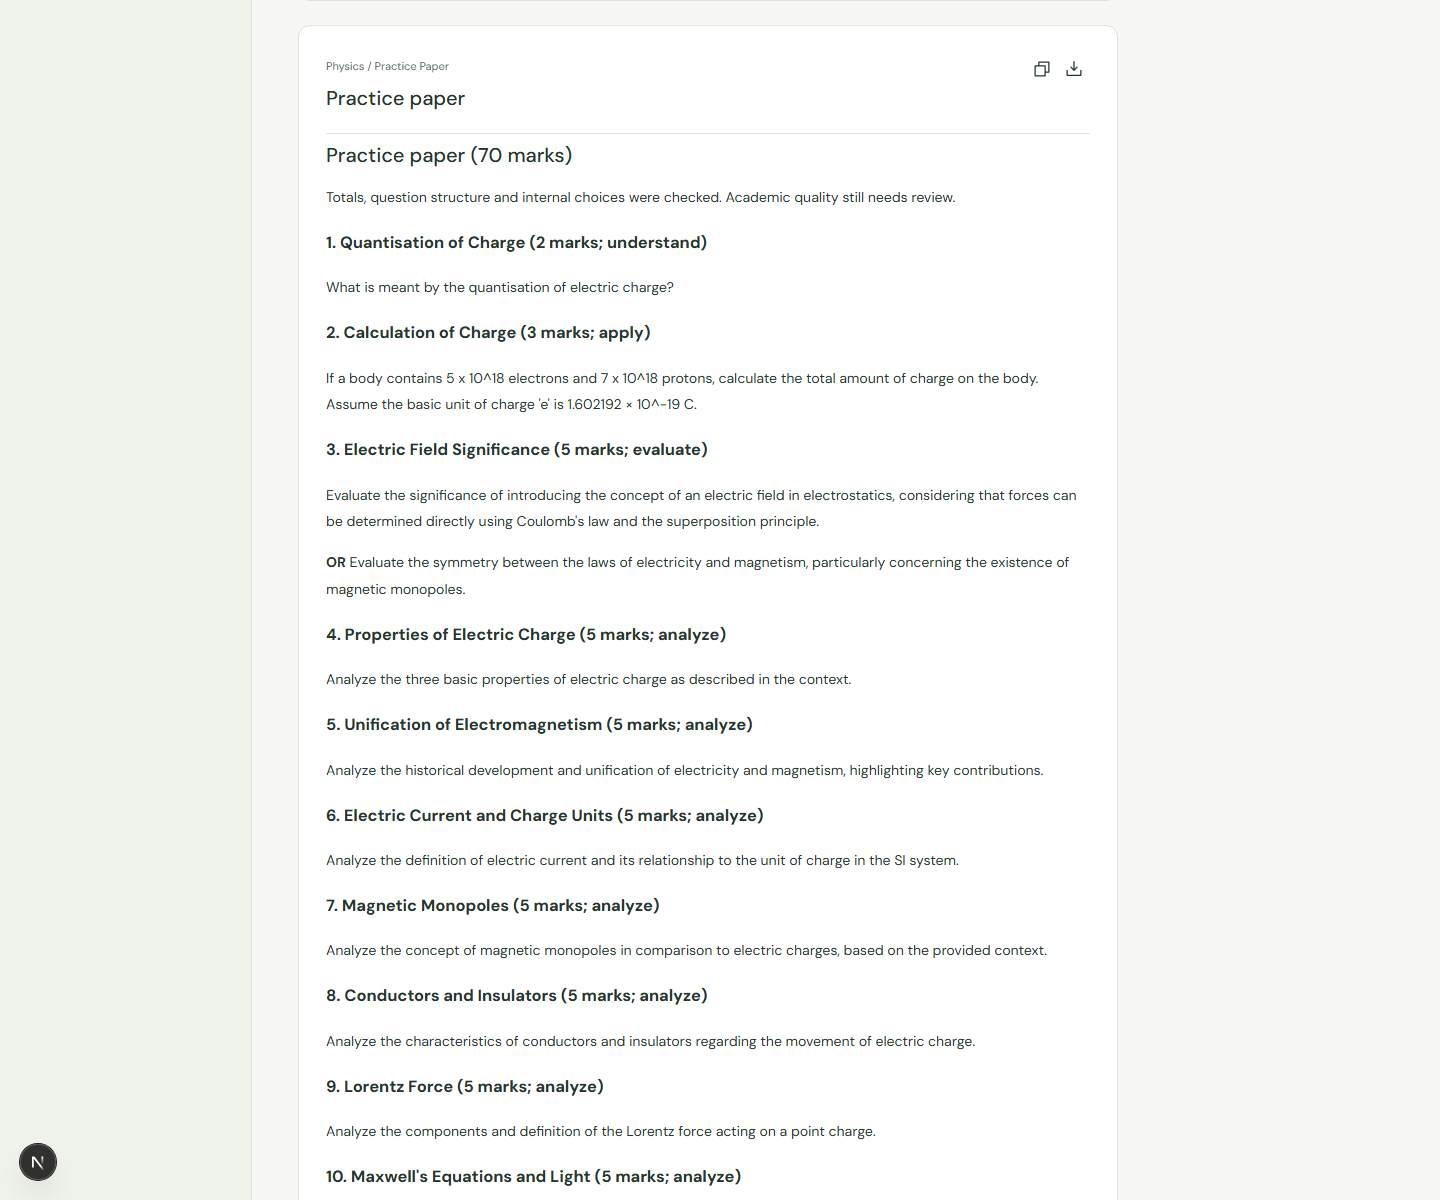
\includegraphics[width=\columnwidth]{figures/r05-mock-result.png}
\caption{Generated 70-mark practice paper (Module~5): ascending Bloom
levels, a worked numeric item, and an internal choice rendered as
\emph{OR}. Generated with Gemini 2.5 Flash on Vertex AI; see
Section~VI-E.}
\label{fig:r-mock}
\end{figure}

\begin{figure}[!t]
\centering
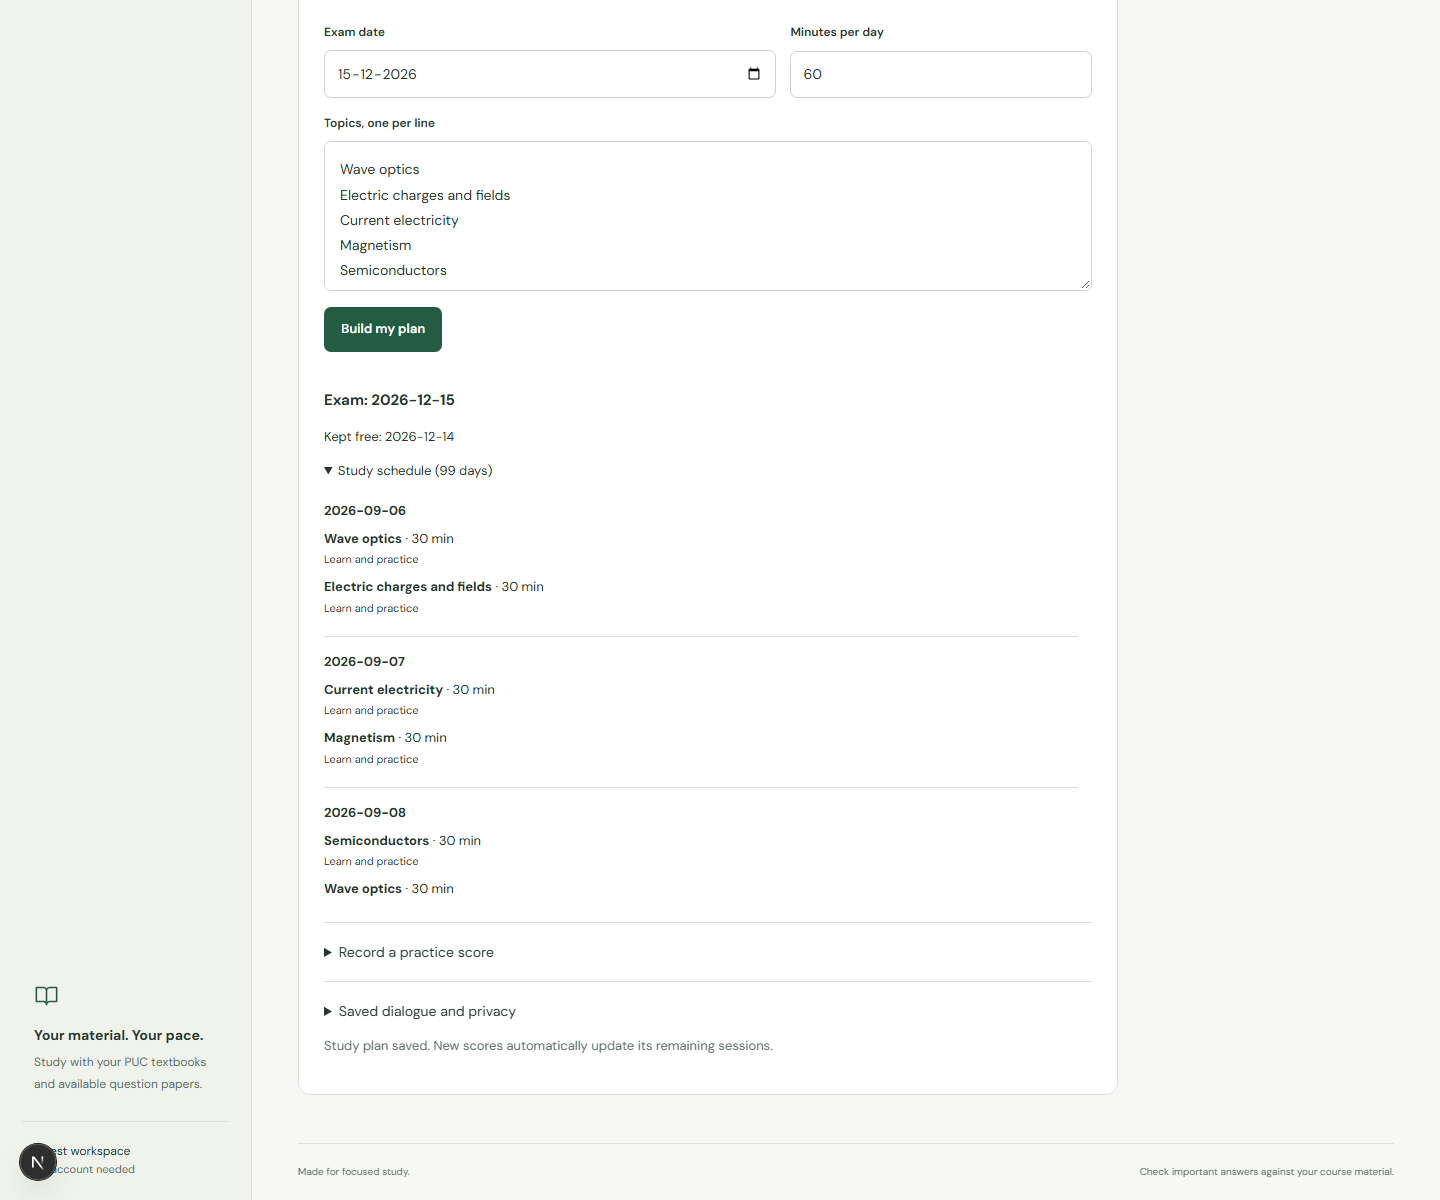
\includegraphics[width=\columnwidth]{figures/r06-planner-result.png}
\caption{Generated 99-day study plan (Module~6), keeping the day before
the exam free.}
\label{fig:r-planner}
\end{figure}

\begin{figure}[!t]
\centering
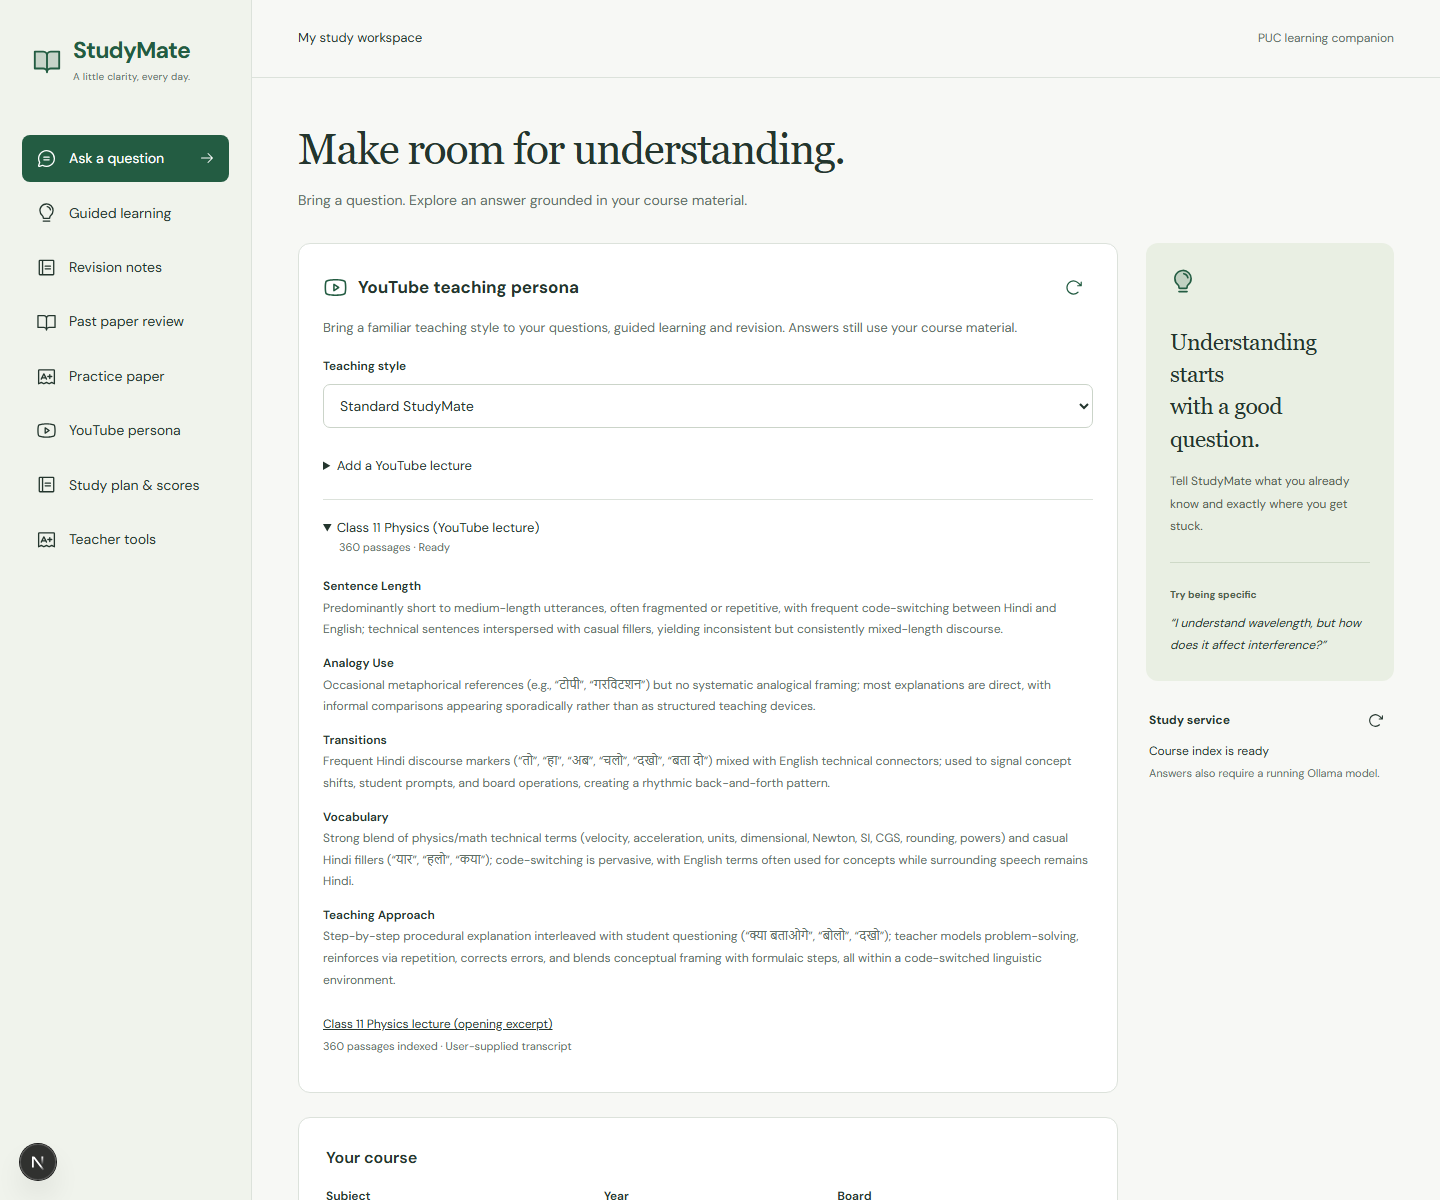
\includegraphics[width=\columnwidth]{figures/r07-persona-fingerprint.png}
\caption{Module~12 style fingerprint distilled from 360 transcript
passages of a registered Class~11 physics lecture, recovering
code-switching, discourse markers, vocabulary mix, and teaching
approach.}
\label{fig:r-persona}
\end{figure}
%------------------------------------------------
\section{Evaluation Framework}
%------------------------------------------------
\subsection{RAGAS Metrics}
Evaluation uses RAGAS~\cite{es2025} on three axes. \textit{Faithfulness}
($F$) is the share of an answer's statements that can be verified
against retrieved context:
\begin{equation}
    F = \frac{V}{S}
\end{equation}
where $V$ is the number of verifiable statements and $S$ the total.
\textit{Answer Relevance} ($AR$) gauges focus by generating $n$
synthetic reverse questions from the answer and averaging their cosine
similarity to the original query $q$:
\begin{equation}
    AR = \frac{1}{n}\sum_{i=1}^{n}\mathrm{sim}(q,\,q_i)
\end{equation}
\textit{Context Relevance} ($CR$) is the fraction of retrieved passages
that were actually relevant, computed as
\begin{equation}
    CR = \frac{R}{K}
\end{equation}
where $R$ is the number of retrieved passages judged relevant to the
query and $K$ is the total number retrieved (top-$k$). The benchmark
comprises 100 questions from five semesters, each vetted by faculty
before inclusion.
\subsection{Persona Style Consistency (PSC)}
PSC tests Module~12's core claim. For each answer under a persona, an
LLM judge sees the answer, three genuine excerpts from the educator, and
three from a neutral baseline, then decides whether phrasing, analogy
use, and sentence structure match the educator. PSC is the share judged
consistent:
\begin{equation}
    PSC = \frac{C}{A}
\end{equation}
with $C$ style-consistent answers out of $A$ total; the target is
$PSC \geq 0.78$.
\subsection{Target Metrics}
Table~\ref{tab:metrics} lists all acceptance thresholds, including PSC.
\begin{table}[htbp]
\caption{Target Evaluation Metrics}
\label{tab:metrics}
\begin{tabular}{ll}
\toprule
\textbf{Metric}                      & \textbf{Target} \\
\midrule
Content Accuracy                     & $\geq 85\%$ \\
RAGAS Faithfulness                   & $\geq 0.85$ \\
RAGAS Answer Relevance               & $\geq 0.80$ \\
RAGAS Context Relevance              & $\geq 0.75$ \\
Persona Style Consistency (PSC)      & $\geq 0.78$ \\
TAM Perceived Usefulness (PU)        & $\geq 4.0/5.0$ \\
TAM Perceived Ease of Use (PEOU)     & $\geq 4.0/5.0$ \\
Response Latency                     & $< 5\,$s \\
PYQ Trend Identification Accuracy    & $\geq 80\%$ \\
Mock Paper Format Compliance         & $\geq 90\%$ \\
Multilingual ASR Word Error Rate     & $\leq 15\%$ \\
\bottomrule
\end{tabular}
\end{table}
\subsection{Technology Acceptance Model}
A TAM survey~\cite{davis1989} will run after at least two weeks of use
with a minimum of 30 respondents. The two-week window is deliberate:
shorter exposure tends to capture novelty rather than considered
utility. The sample is designed to include a fair proportion of
non-English-first students, precisely to avoid the English-fluent
sampling bias common in prior TAM work. A dedicated item asks whether
persona-conditioned replies feel more approachable than standard ones,
giving direct user-acceptance evidence for Module~12.

\subsection{Threats to Validity}
We assess the study against the four standard categories so that
readers can weigh its limits honestly.

\textit{Internal validity.} The strongest threat is the use of an LLM
as judge for both RAGAS and PSC, which can share blind spots with the
generator. We mitigate this by validating a stratified subset of judge
decisions against human faculty ratings and reporting the agreement
rate; systematic divergence would qualify any automated score.

\textit{External validity.} Results come from one institution, a
limited set of subjects, and a cohort of $N \geq 30$, so
generalisation to other curricula, languages, or larger populations is
not guaranteed. The architecture is designed to be re-indexed for other
institutions, but that portability is a claim to be tested, not assumed.

\textit{Construct validity.} PSC operationalises ``sounds like my
lecturer'' through an LLM judge and a $0.78$ threshold calibrated on a
small pilot; the threshold may not transfer across educators with very
different styles, and self-reported TAM usefulness is an imperfect proxy
for actual learning gains, which we do not directly measure here.

\textit{Conclusion validity.} With a modest sample, effect estimates
carry wide confidence intervals, and a two-week window cannot separate
durable adoption from early enthusiasm. We therefore frame all reported
figures as thresholds for a design contribution rather than as
significance claims, and flag a longitudinal study as necessary
follow-up.

\textit{Observations from the running prototype.} Two constraints
surfaced once the system was exercised end to end and qualify the
targets in Table~\ref{tab:metrics}. First, the persona layer and the
multilingual claim interact badly under a single English-trained
encoder: because \texttt{all-MiniLM-L6-v2} embeds an English query far
from Hindi transcript text, a registered Hindi-caption educator never
clears the five-passage floor for an English question, while a Hindi
question fails the course-evidence gate against an English corpus.
Persona conditioning across languages therefore depends on swapping in
a multilingual embedding model, which we treat as required future work
rather than a solved property. Second, generation throughput, not
retrieval, dominates response time, and it is governed by whether the
model fits in GPU memory. On our development host (4-core CPU, RTX~3050
laptop GPU with 4\,GiB of VRAM) a 7B model at 4-bit quantisation needs
about 4.7\,GiB and therefore cannot be resident: Ollama placed it
62\%/38\% across CPU and GPU and sustained 6.5 tokens per second, and
with CUDA unavailable the same model fell to 4.7 tokens per second
entirely on CPU. Qwen2.5-3B occupies roughly 1.9\,GiB, runs 79\% on the
GPU under the same 16{,}384-token context, and sustains 19.6 tokens per
second---a fourfold improvement that motivated our choice of the 3B
variant in Table~\ref{tab:stack}. Even so, the sub-five-second target
in Table~\ref{tab:metrics} is realistic only for short tutoring
answers. A Bloom's-graded paper for 70 marks expands to fifteen
questions plus an answer guide, several thousand generated tokens in
one request, so practice-paper generation is inherently a
tens-of-seconds to minutes operation on commodity hardware. We
therefore treat the latency threshold as applying to interactive
tutoring, and regard progressive streaming or background job delivery
as the appropriate design response for paper generation rather than a
faster decode alone.
%------------------------------------------------
\section{Expected Outcomes and Applications}
%------------------------------------------------
\subsection{Student Benefits}
The first benefit is simply availability: questions that would sit
unanswered until the next lecture can be resolved at once, any hour.
On top of that, students get PYQ trend reports, Bloom's-calibrated
mocks, and a study plan that adjusts to their performance. We expect
the multilingual voice module to drive the single largest adoption gain,
given how many learners struggle with English-only text. The persona
engine adds a different kind of benefit---answers that feel like they
come from a trusted teacher, which the literature on parasocial
learning relationships suggests lowers cognitive friction~\cite{zhao2024}.
\subsection{Teacher Benefits}
The confusion heatmap and query log give near-real-time sight of where
students are stuck, so instructors can adjust before the next
assessment. Registering their own recorded lectures lets faculty push
their teaching voice into the assistant, extending their reach past
contact hours. He et al.~\cite{he2025} reported a 30.3\% UX gain from a
comparable platform, and we expect the persona feature to build on that.
\subsection{Institutional Scalability}
Swapping the four Qdrant collections for another institution's material
yields an equivalent assistant with no LLM retraining, and new personas
are added at runtime through the dashboard. Containerised deployment on
an AWS EC2 t3.medium scales horizontally across departments, and because
inference is local, institution-specific data---conversation logs and
transcripts included---never leaves the institutional server boundary.

\subsection{Contribution to Sustainability}
StudyMate is designed to be sustainable in three concrete senses, which
we make explicit because sustainability shaped several architectural
choices rather than being retrofitted.

\textit{Computational and energy sustainability.} By running a compact
3B model locally via Ollama on a single modest instance instead of
repeatedly calling a large cloud model, the system avoids the
per-query energy and carbon overhead of hyperscale inference. Model
size is a sustainability decision as much as a latency one: the 3B
variant fits within the 4\,GiB of VRAM found on entry-level laptop
GPUs, so the assistant runs on hardware a college already owns rather
than requiring an accelerator purchased for the purpose. The
persona descriptor is cached and refreshed only when new videos are
registered, so expensive style analysis runs once rather than on every
turn, and retrieval gating suppresses wasted generation on
out-of-scope queries. Together these keep the compute footprint low
enough to run on hardware an ordinary college already owns.

\textit{Educational and social sustainability.} The platform maps onto
UN Sustainable Development Goal~4 (quality education) by extending
personalised guidance to students who cannot otherwise reach it, and
onto SDG~10 (reduced inequalities) by serving non-English-first
learners through voice and multilingual support. Rather than replacing
teachers, it amplifies a scarce human resource, which is the more
durable model for under-resourced institutions.

\textit{Operational sustainability.} Because knowledge is stored as
re-indexable text rather than a hand-curated knowledge graph, keeping
the assistant current with an annually changing syllabus costs a
re-ingestion run, not a maintenance project---directly addressing the
upkeep problem that limits KG-based tutors~\cite{dong2025}. Federated
corpus sharing across institutions~\cite{fajardo2025} is a natural next
step for spreading this cost further.
%------------------------------------------------
\section{Conclusion}
%------------------------------------------------
This paper presented StudyMate, a twelve-module Telegram-based RAG
teaching assistant built around nine constraints that converge in
engineering-college classrooms: inaccessible personalised support,
English-only tooling, unused PYQ archives, no adaptive scheduling,
stateless sessions, unencrypted logs, a uniform explanation style, no
Bloom's-aligned mocks, and---most critically---no way to answer in the
voice of a trusted educator. The design addresses all nine within a
single deployable system.

The headline contribution is Module~12, the YouTube Transcript Persona
Engine. By ingesting registered educator transcripts into a dedicated
Qdrant corpus, distilling a lightweight style fingerprint, and
conditioning Qwen2.5-3B on both institutional knowledge and that
fingerprint, StudyMate produces answers that are at once factually
grounded and stylistically familiar. We did not find this capability in
any prior educational RAG system, including
MoodleBot~\cite{neumann2025}, ARIA~\cite{luo2026}, RAG-X~\cite{he2025},
URAG~\cite{nguyen2025}, or the framework of Lauber et al.~\cite{lauber2025}.

Reviewing those systems surfaced the same recurring blind spots: no
regional-language support, no PYQ-based preparation, no encryption, and
no persona conditioning. StudyMate answers all four, and does so with
explicit attention to hallucination control, sustainability, and the
threats that could undermine its own evaluation. The evaluation itself
combines RAGAS faithfulness and relevance, the new Persona Style
Consistency metric, and TAM acceptance on one student cohort, letting
technical performance be read directly against adoption---dimensions
prior studies measured apart. Planned extensions include knowledge
graph augmentation for multi-hop reasoning~\cite{dong2025}, federated
corpus sharing across institutions~\cite{fajardo2025}, and fine-tuning
a smaller on-device model on educator transcripts to push persona
latency below the five-second target.
%------------------------------------------------
\begin{thebibliography}{19}
\bibitem{lewis2020}
P. Lewis et al., ``Retrieval-Augmented Generation for Knowledge-Intensive
NLP Tasks,'' \textit{Adv. Neural Inf. Process. Syst.}, vol. 33,
pp. 9459--9474, 2020.
\bibitem{bloom1984}
B. S. Bloom, ``The 2 Sigma Problem: The Search for Methods of Group
Instruction as Effective as One-to-One Tutoring,'' \textit{Educ.
Researcher}, vol. 13, no. 6, pp. 4--16, 1984.
\bibitem{lauber2025}
A.-M. Lauber, S. Martin, and B. Pampel, ``How Can I Help You? Didactic
Alignment for RAG Chatbots in Education,'' in \textit{Proc. 17th Int.
Conf. Educ. Technol. Comput. (ICETC)}, 2025, pp. 153--158.
\bibitem{teixeira2025}
S. Teixeira, M. Sonkaya, and P. Georgieva, ``RAG Augmented Large
Language Models as a Tool for Education,'' in \textit{Proc. Int. Conf.
Autom. Informatics (ICAI)}, 2025, pp. 769--774.
\bibitem{neumann2025}
A. T. Neumann, Y. Yin, S. Sowe, S. Decker, and M. Jarke,
``An LLM-Driven Chatbot in Higher Education for Databases and
Information Systems,'' \textit{IEEE Trans. Educ.}, vol. 68, no. 1,
pp. 103--112, 2025.
\bibitem{dong2025}
C. Dong, Y. Yuan, K. Chen, S. Cheng, and C. Wen, ``How to Build an
Adaptive AI Tutor for Any Course Using Knowledge Graph-Enhanced
Retrieval-Augmented Generation (KG-RAG),''
\textit{arXiv preprint arXiv:2311.17696}, 2025.
\bibitem{nguyen2025}
L. Nguyen and T. Quan, ``URAG: Implementing a Unified Hybrid RAG for
Precise Answers in University Admission Chatbots,''
\textit{arXiv preprint arXiv:2501.16276}, 2025.
\bibitem{zhao2024}
Z. Zhao, Z. Yin, J. Sun, and P. Hui, ``Embodied AI-Guided Interactive
Digital Teachers for Education,'' in \textit{SIGGRAPH Asia Educators
Forum}, ACM, 2024.
\bibitem{he2025}
S. He, L. Liu, J. Ma, and Y. Lu, ``RAG-X-Driven Construction of an
Intelligent Platform for Teaching Assistance in Higher Education,''
in \textit{Proc. 5th Int. Conf. Educ. Technol. (ICET)}, 2025,
pp. 238--242.
\bibitem{luo2026}
Y. Luo, D. R. Sarkar, R. H. Sangree, and S. Goswami,
``ARIA: Adaptive Retrieval Intelligence Assistant---A Multimodal RAG
Framework for Domain-Specific Engineering Education,''
\textit{arXiv preprint arXiv:2604.06179}, 2026.
\bibitem{koutsiaki2025}
M. E. Koutsiaki et al., ``From Textbook to Talkbot: A Case Study of a
Greek-Language RAG-Based Chatbot in Higher Education,'' in
\textit{Proc. Barcelona Conf. Educ.}, 2025.
\bibitem{gielis2025}
A. Gielis et al., ``Personalized Self-Assessment Tool Using a Telegram
Bot: A Case Study on Data Structures and Algorithms,''
\textit{arXiv preprint arXiv:2601.06225}, 2025.
\bibitem{es2025}
S. Es, J. James, L. Espinosa-Anke, and S. Schockaert,
``RAGAS: Automated Evaluation of Retrieval Augmented Generation,''
\textit{arXiv preprint arXiv:2309.15217}, 2025.
\bibitem{davis1989}
F. D. Davis, ``Perceived Usefulness, Perceived Ease of Use, and User
Acceptance of Information Technology,'' \textit{MIS Quart.}, vol. 13,
no. 3, pp. 319--340, 1989.
\bibitem{roh2021}
Y. Roh, G. Heo, and S. E. Whang, ``A Survey on Data Collection for
Machine Learning: A Big Data--AI Integration Perspective,''
\textit{IEEE Trans. Knowl. Data Eng.}, vol. 33, no. 4,
pp. 1328--1347, 2021.
\bibitem{kuhail2023}
M. A. Kuhail et al., ``Interacting with Educational Chatbots: A
Systematic Review,'' \textit{Educ. Inf. Technol.}, vol. 28, no. 1,
pp. 973--1018, 2023.
\bibitem{wollny2021}
A. Wollny et al., ``Are We There Yet? A Systematic Literature Review on
Chatbots in Education,'' \textit{Front. Artif. Intell.}, vol. 4,
p. 654924, 2021.
\bibitem{fajardo2025}
V. A. Fajardo et al., ``FedRAG: A Framework for Fine-Tuning
Retrieval-Augmented Generation Systems,''
\textit{arXiv preprint arXiv:2506.09200}, 2025.
\bibitem{li2023}
Y. Li et al., ``Style-Conditioned Language Generation for Personalized
Dialogue,'' in \textit{Proc. ACL}, 2023, pp. 4810--4824.
\end{thebibliography}
\end{document}
